\documentclass[12pt]{article}

% ---------- Fonts ----------
\usepackage{newtxtext,newtxmath}   % Times New Roman text + math

% ---------- Layout ----------
\usepackage[margin=1in]{geometry}
\usepackage{setspace}
\onehalfspacing
\setlength{\parskip}{6pt}
\usepackage{placeins}
\usepackage{float}
\usepackage{graphicx}
% ---------- Tables ----------
\usepackage{booktabs}
\usepackage{array}
\usepackage{siunitx}
\usepackage{indentfirst}

% ---------- Math / symbols ----------
\usepackage{amsmath, amssymb}
\usepackage{caption}
\captionsetup{skip=8pt}
\renewcommand{\arraystretch}{1.25}

% ---------- Hyperlinks ----------
\usepackage[hidelinks]{hyperref}

% ---------- Citations ----------
\usepackage[numbers,sort&compress]{natbib}
\bibliographystyle{ieeetr}

% ---------- Title ----------
\title{Bayesian Optimization of Microfluidic Tumor-on-Chip Geometry for a Linear Drug-Concentration Gradient: A Topology-First Design Methodology}
\author{Shuo Li, Xiaoyu Wang}


\begin{document}
\maketitle

% =========================================================
\begin{abstract}
% =========================================================
We propose a topology-first inverse-design framework for microfluidic tumor-on-chip chambers that produce a prescribed linear drug-concentration gradient. The framework couples parametric \texttt{blockMesh} geometry generation, two-stage OpenFOAM CFD (\texttt{simpleFoam} momentum + \texttt{scalarTransportFoam} scalar transport), and a constrained Bayesian-optimization (BO) loop with five Gaussian-process constraint surrogates encoding biology, manufacturability, and laminar-regime limits. Eight topologies were considered in total: three two-inlet baselines (\emph{opposing}, \emph{same-side Y}, \emph{asymmetric lumen}) carried over from the first design trial against an axis-$x$ target, plus five novel candidates screened in the second trial; of those, the stacked ladder was implemented and benchmarked end-to-end while the remaining four (Christmas-tree mixer, distributed side injection, permeable wall, counter-flow) were ruled in or out from first principles. The methodological observation underlying the topology pivot is that mass conservation furnishes a closed-form admissibility test that should be applied \emph{before} any optimization: in laminar two-inlet coflow, a streamwise linear gradient is mathematically forbidden, so a $600$-evaluation BO campaign over the three two-inlet baselines necessarily plateaus at a $0.585$ uniform-field floor regardless of acquisition strategy. The cross-topology BO comparison against an axis-$y$ linear target lifts the ladder winner to $L_2 = 0.082$, $R^2 = 0.987$ at $H = 200~\mu$m, beating the next-best two-inlet topology by $10.8\times$ on the same target. A height sweep further reduces the ladder error to $L_2 = 0.067$, $R^2 = 0.990$ at $H = 300~\mu$m, with feasibility leaping from $37\%$ to $96.5\%$. A subsequent ablation that unmasks the pillar parameters $(d_p, s_p)$ uncovers a regime swap: introducing even a single $1\!\times\!4$ pillar row drops $S_T(Q_{\text{total}})$ from $0.87$ to $0.001$ and surfaces $s_p$ as the second-most-important lever, with the best design dropping a further $\sim 30\%$ in $L_2$. Beyond the optima, the trained surrogates yield three reusable interpretability outputs: cross-topology Sobol total-effect indices that reveal $r_{\text{flow}}$ as a universal driver of the two-inlet class, the inlet convergence angle $\theta$ as consistently inactive, and a $W \rightleftarrows Q_{\text{total}}$ trade-off as the secondary lever; bisection-based fabrication-tolerance intervals; and constraint-binding diagnostics that telegraph the next experimental investment. Together these constitute a transferable design-of-experiments methodology for any prescribed-field laminar-microfluidic problem, with the optimization itself acting as the engine that produces interpretable design recommendations and manufacturability guidance.
\end{abstract}

% =========================================================
\section{Introduction}
% =========================================================
Microfluidic tumor-on-chip (ToC) systems are \textit{in vitro} platforms that recreate key features of the tumor microenvironment by integrating living cells within precisely controlled microfluidic architectures. Pairing microfabrication with 3D cell culture, they cast spatial and temporal control over biochemical and mechanical cues---fluid flow, nutrient transport, drug exposure---and, compared with two-dimensional culture or animal models, deliver improved physiological relevance while remaining experimentally tractable. They have therefore become a promising tool for studying cancer progression and therapeutic response~\cite{liu2021tumor}.

Among the defining features of the tumor microenvironment are spatial gradients in soluble factors such as oxygen, nutrients, and drugs. Such gradients arise from the interplay of transport processes and cellular consumption, and they shape cell proliferation, metabolism, and drug sensitivity~\cite{guerrero2026matrix}. Drug-concentration gradients are particularly central to understanding heterogeneous treatment responses, since cells within the same tumor may experience widely different exposure levels; reproducing them \textit{in vitro} is therefore essential for building predictive models of therapeutic efficacy~\cite{shen2020concentration}.

Microfluidic gradient generators have been developed widely to address this need, leveraging laminar flow and diffusion to sculpt controlled concentration fields. Classical layouts come in several flavours---tree-like binary mixers (the ``Christmas tree'' introduced by Whitesides and colleagues and refined by Dertinger), Y-junctions, side-by-side coflow chambers with central tongues, and asymmetric lumen configurations---each producing a stepwise distribution that approximates a continuous gradient across a chamber. Their simplicity and robustness has made them a standard tool in microfluidics, particularly for biological assays requiring graded chemical environments~\cite{jeon2000generation,dertinger2001generation,ayuso2021microfluidic}.

Despite their widespread adoption, existing gradient-generation strategies are typically arrived at by forward design: geometry and flow conditions are tuned manually using human intuition or empirical heuristics. This limits how precisely a target profile can be reproduced, especially in tumor-on-chip systems where geometric, manufacturability, and biological constraints have to be satisfied simultaneously. Recent work has begun to move toward optimization-based design. Yang et al.\ proposed a Kriging surrogate with adaptive sampling for prescribed-gradient generators~\cite{yang2020surrogate}; Hong et al.\ introduced a deep neural network for inverse design~\cite{hong2020inverse}; Zhang et al.\ assembled an ML-enabled framework that accelerates evaluation by $300\times$ over conventional finite-element analysis~\cite{zhang2022machine}; Kundacina et al.\ have applied Bayesian optimization to general microfluidic device design~\cite{kundacina2025advancing}. These works share two assumptions, however: that the desired concentration profile is physically attainable within the chosen topology, and that interpretability of the resulting surrogate is a secondary concern. None addresses whether a given topology imposes fundamental limits on achievable concentration fields independent of the optimization strategy, and none reports the kind of cross-topology sensitivity comparison, fabrication-tolerance intervals derived from a CFD-trained surrogate, or dimensional-physics constraint set wired into the acquisition function that a tumor-on-chip 3D-culture chamber actually demands.

A critical but under-explored question is therefore whether a given microfluidic topology can, in principle, realise a prescribed concentration field. In laminar microfluidic systems with coflowing streams, transport is governed by advection--diffusion and constrained by mass conservation; these constraints impose fundamental limits on achievable distributions independent of any tuning or optimization strategy~\cite{stone2004engineering}. Failing to account for them can lead to misleading optimization outcomes in which an algorithm appears to converge but is in fact bounded by a physical impossibility rather than its compute budget.

In this work we address this gap by formulating the tumor-on-chip gradient design problem as an inverse problem and combining CFD with constrained Bayesian optimization to explore both parametric and topological design spaces. Beyond locating an optimum, we exploit the trained Gaussian-process surrogate for a \emph{post-hoc interpretability triple}: Sobol total-effect indices rank parameter influence; local-sensitivity gradients confirm the ranking at the optimum; bisection-based tolerance intervals bound fabrication and operational drift; and a constraint-binding diagnostic identifies the active feasibility ``shortest staves''---the constraints that limit performance while others retain slack. We then demonstrate that two-inlet coflow geometries are inherently incapable of generating a streamwise linear gradient under these transport equations and pivot to a stacked-ladder topology aligned with the natural transverse transport structure, achieving an order-of-magnitude reduction in $L_2$ over the two-inlet baseline and a further $\sim 18\%$ improvement via chamber-height relaxation. A subsequent pillar-ablation campaign re-opens two design dimensions previously masked by an a-priori assumption and reveals an additional $\sim 30\%$ headroom together with a regime swap in the dominant control variable. Three contributions follow: (i) a mass-conservation \emph{feasibility pre-screen} as a generalisable methodological tool, (ii) a constraint-aware BO with five GP constraint surrogates and a dimensional-physics diagnostic-metric set, and (iii) the post-hoc interpretability triple that turns optimization output into actionable experimental guidance.

% =========================================================
\section{Method}
% =========================================================

\subsection{Eight Topologies and Two Design Trials}
\label{sec:eight_topologies}
The study spans two design trials, eight topologies in total. Trial~1 ran a $600$-evaluation BO campaign on the three two-inlet baselines (\emph{opposing}, \emph{same-side Y}, \emph{asymmetric lumen}) against an axis-$x$ linear target; the result diagnosed a topology-class limit (Section~\ref{sec:original_three}) and motivated five replacement candidates. Trial~2 introduced these five candidates and ran the cross-topology comparison against an axis-$y$ target. Four of the five (Christmas-tree mixer, distributed side injection, permeable wall, counter-flow) were ruled in or out by first-principles physical analysis of mass conservation, manufacturability, and steady-state existence (Section~\ref{sec:topology_screening}); the fifth, the stacked ladder, was implemented end-to-end and benchmarked under the same constraint set as the three baselines. A height sweep ($H \in \{200, 300\}~\mu$m) and a pillar ablation ($\text{pillar\_config} \in \{\text{none}, 1\!\times\!4\}$) follow on the ladder topology. Table~\ref{tab:topology_overview} maps each topology to its trial, target axis, and the type of analysis applied.

\begin{table}[H]
\centering
\caption{The eight topologies considered in this study, mapped to the trial in which each was investigated, the target gradient axis, and the kind of analysis applied. ``BO'' denotes a full BoTorch CEI campaign with $\geq 100$ evaluations; ``screened'' denotes first-principles admissibility analysis without CFD enumeration.}
\label{tab:topology_overview}
\begin{tabular}{l c c l}
\toprule
\textbf{Topology} & \textbf{Trial} & \textbf{Target axis} & \textbf{Analysis} \\
\midrule
Opposing                  & 1, 2 & $x$, $y$ & BO, $H{=}200$ (axis-$x$ + axis-$y$) \\
Same-side Y               & 1, 2 & $x$, $y$ & BO, $H{=}200$ (axis-$x$ + axis-$y$) \\
Asymmetric lumen          & 1, 2 & $x$, $y$ & BO, $H{=}200$ (axis-$x$ + axis-$y$) \\
\textbf{Ladder}           & 2 & $y$ & BO, $H{=}200,300$; pillar ablation $H{=}200$ \\
Christmas-tree mixer      & 2 & $y$ & screened only (admissible; future work) \\
Distributed side injection& 2 & $x$ & screened only (sole admissible axis-$x$ route) \\
Permeable wall            & 2 & $x$ & screened only (admissible; requires membrane model) \\
Counter-flow              & 2 & $x$ & screened only (steady-state conditional on Re) \\
\bottomrule
\end{tabular}
\end{table}

\subsection{Parametric Geometry and Design Space}
The tumor-on-chip chamber is modelled as a rectangular conduit of fixed streamwise length $L = 10$~mm, chosen to accommodate standard 3D cell-culture volumes while remaining compatible with soft-lithographic fabrication~\cite{ayuso2021microfluidic}. Seven continuous geometric and flow variables make up the parametric design space (Table~\ref{tab:design_space}); the variables were selected for their established influence on advective--diffusive transport in laminar microfluidics and their practical manufacturability within polydimethylsiloxane (PDMS) soft lithography.

The chamber height $H$ is treated as a discrete parameter at $200~\mu$m or $300~\mu$m, fixed for a given optimization campaign. This range is consistent with established PDMS-based tumor-on-chip platforms supporting three-dimensional cell culture. The aspect ratio $W/H$ is constrained \emph{a posteriori} to $\leq 15$ to forestall irreversible PDMS-channel collapse during plasma bonding, a recognised failure mode for shallow, wide channels~\cite{xia1998}.

\begin{table}[htbp]
\centering
\caption{Parametric design space. The rightmost column lists which topology / pillar configurations activate each parameter at the BO layer; masked dimensions are pinned to the midpoint of their bounds and are not optimised. The pillar-ablation campaign of Section~\ref{sec:pillar_ablation} unmasks $d_p$ and $s_p$ for the ladder when \texttt{pillar\_config} $\neq$ \texttt{none}.}
\label{tab:design_space}
\begin{tabular}{l c l c p{3.6cm} l}
\toprule
\textbf{Parameter} & \textbf{Symbol} & \textbf{Unit} & \textbf{Range} & \textbf{Description} & \textbf{Active in} \\
\midrule
Chamber width            & $W$              & $\mu$m       & $[1500, 4500]$ & Transverse dimension perpendicular to mean flow & all \\
Total flow rate          & $Q_{\text{total}}$ & $\mu$L/min & $[5, 200]$    & Combined inlet volumetric flow rate              & all \\
Inlet flow ratio         & $r_{\text{flow}}$ & ---        & $[0.10, 0.97]$& Drug fraction $Q_{\text{drug}}/Q_{\text{total}}$ & two-inlet trio \\
Inlet convergence angle  & $\theta$         & deg          & $[15, 75]$    & Half-angle between inlet channels at junction    & two-inlet trio \\
Tongue offset            & $\delta_{W}$     & ---          & $[0.12, 0.48]$& Normalised offset of dividing tongue             & opposing only \\
Pillar diameter          & $d_{p}$          & $\mu$m       & $[100, 400]$  & Diameter of cylindrical stagnation pillars       & pillar configs only \\
Pillar spacing           & $s_{p}$          & $\mu$m       & $[200, 1000]$ & Centre-to-centre pillar spacing                  & pillar configs only \\
\bottomrule
\end{tabular}
\end{table}

For the bare ladder ($\text{pillar\_config} = \text{none}$), the geometry is fully specified by $(W, H, N, \text{convention})$ and the operating point by $Q_{\text{total}}$; the other five parameters in Table~\ref{tab:design_space} have no mechanical role (no pillars, no inlet-angle junction, no tongue offset, no two-stream flow split) and are masked at the BO layer. The bare-ladder optimisation is therefore a 2-D constrained BO in $(W, Q_{\text{total}})$. The pillar ablation of Section~\ref{sec:pillar_ablation} re-activates $d_p$ and $s_p$ once any pillar configuration is chosen, lifting the search to 4-D in $(W, d_p, s_p, Q_{\text{total}})$.

Three baseline two-inlet topologies were initially constructed. The \emph{opposing} configuration positions two inlets at $x = 0$ on opposite short-side walls separated by a central dividing tongue. The \emph{same-side Y} topology merges two inlet streams via a Y-junction upstream of the chamber entrance, with each branch occupying half the chamber height. The \emph{asymmetric-lumen} topology, adapted from Ayuso et al., introduces a side-wall lumen that generates a transverse gradient across the central culture region~\cite{ayuso2021microfluidic}. Each is implemented as a parametric \texttt{blockMeshDict} generator within OpenFOAM, allowing programmatic mesh construction for any admissible parameter combination.

The fourth topology---the \emph{ladder}---was added during Trial~2 (Section~\ref{sec:topology_screening}). Originally demonstrated by Jeon et al.\ and Dertinger et al.~\cite{jeon2000generation,dertinger2001generation}, the ladder lays out $N$ stacked inlet strips at $x = 0$, each delivering a prescribed concentration $C_k$ ($k = 0, \dots, N-1$); the resulting gradient lies in the transverse ($y$) direction. We use $N = 8$ throughout, the smallest discretisation for which the $L_2$ error has saturated empirically (Section~\ref{sec:ladder_diagnostic}). Strip concentrations follow the midpoint convention $C_k = (k + 0.5)/N$, which centres each strip on the linear target and reduces step-quantisation error by $38\%$ relative to the more common endpoint convention $C_k = k/(N-1)$.

\subsection{Mass-Conservation Feasibility Pre-screen}
\label{sec:mass_conservation}
Before any optimization, mass conservation supplies a closed-form admissibility test for whether a topology can in principle realise a prescribed gradient. Define the depth-averaged concentration $\langle C \rangle_y(x) = (1/W)\int_0^W C(x,y)\, dy$. Integrating the steady-state advection--diffusion equation $\nabla \cdot (\mathbf{U}C - D\nabla C) = 0$ across the chamber width with no-flux side-wall boundary conditions yields
\begin{equation}
\frac{d}{dx}\!\left[\frac{1}{W}\!\int_0^W u(x,y)\, C(x,y)\, dy\right] = 0,
\label{eq:mc_constancy}
\end{equation}
i.e.\ the streamwise advective flux of $C$ is constant along the chamber. For an approximately uniform velocity profile (laminar, fully developed) this collapses to $\langle C \rangle_y(x) = \text{const}$. Evaluating at $x=0$ for a two-inlet coflow with $c_{\text{low}} = 0$, $c_{\text{high}} = 1$:
\begin{equation}
\langle C \rangle_y(x) \;=\; r_{\text{flow}} \quad \forall x \in [0, L].
\label{eq:rflow_constancy}
\end{equation}
A linear-$x$ target $\langle C \rangle_y(x) = x/L$ varies with $x$ and is therefore mathematically incompatible with Eq.~\ref{eq:rflow_constancy} for any choice of geometry or flow. The corresponding $L_2$ floor is set by the deviation of a uniform field at $C = r_{\text{flow}}$ from the linear target; numerically, $L_2^{\text{floor}} \approx 0.585$ at $r_{\text{flow}} = 0.5$. The chamber's natural concentration structure is transverse ($y$-direction stratification with diffusive smoothing), not streamwise. The argument applies to any prescribed-streamwise-gradient design problem under laminar two-inlet coflow, independent of the optimization strategy chosen on top of it. Table~\ref{tab:admissibility} converts the argument into a reusable admissibility table by topology class and target shape.

\begin{table}[htbp]
\centering
\caption{Mass-conservation admissibility pre-screen. ``$\checkmark$'' = admissible at first principles; ``$\times$'' = forbidden by Eq.~\ref{eq:rflow_constancy}; ``---'' = degenerate or trivially admissible. The pre-screen should be applied before any BO campaign.}
\label{tab:admissibility}
\begin{tabular}{l c c c c}
\toprule
& \textbf{linear-$x$} & \textbf{linear-$y$} & \textbf{step-$y$} & \textbf{bimodal-$y$} \\
\midrule
Two-inlet coflow (opposing, SSY, asym.\ lumen) & $\times$ & $\checkmark$ (limited) & $\checkmark$ & $\times$ \\
Imposed-inlet ladder ($N$ strips, $N \geq 3$)   & $\times$ & $\checkmark$ & $\checkmark$ & $\checkmark$ \\
Distributed source (side-injection, permeable wall) & $\checkmark$ & --- & $\checkmark$ & $\checkmark$ \\
Counter-flow                                    & $\checkmark$ & $\times$ & unsteady & unsteady \\
\bottomrule
\end{tabular}
\end{table}

\subsection{Computational Fluid Dynamics Framework}
Each candidate geometry is evaluated using steady-state CFD in OpenFOAM v2406~\cite{weller1998tensorial,jasak2009openfoam}. Velocity is solved with \texttt{simpleFoam} (the SIMPLE algorithm for incompressible laminar steady flow):
\begin{equation}
\nabla \cdot \mathbf{U} = 0, \qquad \mathbf{U} \cdot \nabla \mathbf{U} = -\frac{1}{\rho} \nabla p + \nu \nabla^2 \mathbf{U},
\end{equation}
with $\rho = 1000~\text{kg/m}^3$, $\nu = 1\times 10^{-6}~\text{m}^2/\text{s}$, no-slip walls, prescribed inlet velocity profiles, and zero-gauge outlet pressure~\cite{ferziger2012}. Scalar transport of a passive drug surrogate is then solved on the converged velocity field with \texttt{scalarTransportFoam}:
\begin{equation}
\mathbf{U} \cdot \nabla C = D \nabla^2 C, \qquad D = 1\times 10^{-10}~\text{m}^2/\text{s},
\end{equation}
representative of fluorescein-class small-molecule diffusivity in water~\cite{chenyakin2017diffusion}. Inlet concentrations are $C_{\text{drug}} = 1.0$ at the drug inlet and $C_{\text{medium}} = 0.0$ at the medium inlet (or per-strip values for the ladder).

The mesh is generated with \texttt{blockMesh}; production runs use structured hexahedral cells at \emph{20 cells per millimetre} in both $x$ and $y$. As a concrete check: the $H = 300$ winner case ($W = 4495.6~\mu$m, eight inlet strips of width $561.95~\mu$m) carries $200$ cells in $x$ over $L = 10$~mm and $11 \times 8 = 88$ cells in $y$ over $W$, giving $11$ cells per inlet strip. The resolution choice is supported by two verification studies described below.

\paragraph{Solver verification (1-D advection--diffusion).} \texttt{scalarTransportFoam} was checked against the textbook analytic solution
\begin{equation}
C(\xi) = \frac{1 - \exp\!\big( -\text{Pe}\,(1 - \xi) \big)}{1 - \exp(-\text{Pe})}, \qquad \xi = x/L,
\label{eq:ad_analytic}
\end{equation}
on a 1-D channel with uniform velocity, at four P\'eclet numbers spanning the design-relevant regime. Table~\ref{tab:scalar_verification} records the results; all four cases pass a $2\%$ relative-$L_2$ tolerance. Pe$=1000$ required $n = 500$ cells (a $100$-cell mesh fails the bar at this Pe because of upwind numerical diffusion---a regime that the production runs avoid).

\begin{table}[H]
\centering
\caption{Solver verification of \texttt{scalarTransportFoam} against the 1-D advection--diffusion analytic solution (Eq.~\ref{eq:ad_analytic}).}
\label{tab:scalar_verification}
\begin{tabular}{c c c c c}
\toprule
$\text{Pe}$ & $n_{\text{cells}}$ & $L_2$ rel.\ error & $L_\infty$ error & Pass \\
\midrule
1     & 100 & $0.064\%$ & $0.058\%$ & \checkmark \\
10    & 100 & $0.77\%$  & $1.63\%$  & \checkmark \\
100   & 100 & $1.26\%$  & $10.65\%$ & \checkmark \\
1000  & 500 & $1.66\%$  & $36.79\%$ & \checkmark \\
\bottomrule
\end{tabular}
\end{table}

\paragraph{Mesh-convergence study (Hagen--Poiseuille).} A separate convergence study refines the velocity-field mesh on a fixed Hagen--Poiseuille channel geometry at $n_x \in \{100, 200, 400\}$ ($n_y \in \{10, 20, 40\}$); the mean-velocity errors against the analytic parabolic profile are $1.18\%$, $0.39\%$, and $0.13\%$, respectively. The production resolution of $20$ cells/mm therefore lies on the converged plateau; further refinement recovers about $0.4\%$ in velocity and is reserved for publication-quality reruns (Section~\ref{sec:limits_future}).

For each evaluation, momentum convergence is declared once residuals fall below $10^{-6}$ for $100$ additional iterations; the scalar solver is considered converged at $C$-residual $< 10^{-7}$. Non-converged runs are terminated at $2000$ (\texttt{simpleFoam}) or $500$ (\texttt{scalarTransportFoam}) iterations and flagged as penalty observations. A single evaluation requires roughly $12$~s of wall time on a single core (Apple~M4); the four-topology / 200-evaluations-per-topology integration campaign of Section~\ref{sec:bo_h200} completes in $\sim 1$~h on an 8-core workstation, and the ladder-only $H = 200$ vs $H = 300$ height sweep ($2 \times 200$ evaluations) finishes in $13$~min~$22$~s.

\subsection{Bayesian Optimization Framework}
The design space is explored using constrained BO implemented with BoTorch. A Gaussian-process surrogate with a Mat\'ern-5/2 kernel models the mapping from the parameter vector $\mathbf{x}$ to the objective $L_2(\mathbf{x})$~\cite{balandat2019botorch,rasmussen2008gp}. The surrogate is initialised with $24$ Sobol-sequence samples to seed uniform coverage of the parameter space.

Acquisition uses Constrained Expected Improvement over a \texttt{ModelListGP} containing one GP for the objective (minimised) and five independent GPs for the constraints described in Section~\ref{sec:constraints}. At each iteration the acquisition is optimised by L-BFGS-B with ten random restarts to pick the next candidate $\mathbf{x}_{\text{next}}$~\cite{gardner2014boic}; the candidate is evaluated by the CFD pipeline and all surrogates updated.

\emph{Topology is treated as a categorical hyperparameter}: we run an independent BO loop per topology with a shared parameter space and constraint set, then compare optima across topologies. Each loop runs for $200$ evaluations (or $100$, in the pillar-ablation campaign of Section~\ref{sec:pillar_ablation}); the winner is the feasible evaluation with the lowest $L_2$. The trained GP surrogates are preserved for the post-hoc interpretability analysis of Section~\ref{sec:interpretability_methods}, so additional CFD calls are not needed at the analysis stage.

The objective $L_2$ and the auxiliary $R^2$-to-linear metric are defined as
\begin{equation}
L_2 \;=\; \frac{\| C - C_{\text{target}} \|_2}{\| C_{\text{target}} \|_2},
\qquad
R^2_{\text{lin}} \;=\; 1 - \frac{\sum_y \big( \langle C \rangle_x(y) - (a + b\, y/W) \big)^2}{\sum_y \big( \langle C \rangle_x(y) - \overline{C} \big)^2},
\label{eq:l2_r2}
\end{equation}
where $(a, b)$ are the least-squares coefficients of a linear fit to the depth-averaged $\langle C \rangle_x(y)$ along the midline. $L_2$ conflates magnitude and shape errors, whereas $R^2_{\text{lin}}$ isolates shape independently of offset and dynamic range; the two diverge when comparing fields of differing $C_{\text{std}}$, and reporting both makes the difference legible.

\subsection{Constraints and Feasibility}
\label{sec:constraints}
A design is feasible only if all five constraints in Table~\ref{tab:constraints} are satisfied. The set was assembled to span four orthogonal experimental concerns---biology, flow uniformity, laminar-regime safety, manufacturability---plus one discrete experimental knob (chamber height fixed per campaign). It is not the only possible set, but each constraint earns its place by addressing a different practitioner concern.

\begin{table}[H]
\centering
\caption{Constraint definitions and threshold values. All are computed from CFD and encoded as independent Gaussian processes within the \texttt{ModelListGP} acquisition.}
\label{tab:constraints}
\begin{tabular}{l c c p{5cm}}
\toprule
\textbf{Constraint} & \textbf{Symbol} & \textbf{Threshold} & \textbf{Justification} \\
\midrule
Mean wall shear stress & $\tau_{\text{mean}}$ & $[0.1, 2.0]$~Pa & Lower bound prevents flow stagnation; upper bound prevents shear-induced cell detachment \\
Dead-zone fraction & $f_{\text{dead}}$ & $\leq 0.08$ & Fraction of the developed-flow region with velocity below $10\%$ of the region-mean magnitude; ensures flow uniformity \\
Reynolds number & $\text{Re}$ & $\leq 100$ & Guarantees laminar flow regime ($\text{Re} = \rho U_{\text{avg}} D_h / \mu$) \\
Aspect ratio & $W/H$ & $\leq 15$ & Prevents PDMS channel collapse during plasma bonding \\
Chamber height & $H$ & $200$ or $300~\mu$m & Discrete parameter fixed per campaign \\
\bottomrule
\end{tabular}
\end{table}

The aspect-ratio cap of $15$ sits within the literature consensus range $10$--$20$ for reliable PDMS bonding~\cite{xia1998} and gives the BO a little headroom over the conservative literature canonical of $10$. The shear cap of $2.0$~Pa is appropriate for tolerant cell lines (immortalised lines, hepatocytes, endothelial cells, $2$--$5$~Pa for hours). Sensitive cell lines (primary tumour cells, neurons) may require tightening to $1.0$~Pa, in which case the $H = 300$ winner remains feasible while the $H = 200$ winner does not (see Section~\ref{sec:constraint_assessment}). The Reynolds cap is a safety rail---across $1200$ evaluations the maximum observed $\text{Re}$ was $41.7$---and the dead-zone cap turns out to be the dominant cause of infeasibility for the asymmetric lumen, whose stagnant-corner geometry is structurally hard to escape.

\subsection{Topology Screening and Ladder Implementation}
\label{sec:topology_screening}
The Trial~1 campaign confirmed that the original three two-inlet topologies cannot produce a streamwise-linear gradient (Section~\ref{sec:original_three}). To overcome the limit, five replacement candidates were screened from first principles in Trial~2:
\begin{itemize}
\item \emph{A. Stacked ladder} ($N$ y-strips at $x = 0$, prescribed $C_k$). Whitesides--Dertinger ancestry; target axis $y$. Cheapest to implement; aligned with the mass-conservation argument; selected for full implementation.
\item \emph{B. Christmas-tree mixer.} Binary mixing tree feeding $N$ chamber inlets~\cite{dertinger2001generation,yang2020surrogate}; admissible by Table~\ref{tab:admissibility}. Future work.
\item \emph{C. Distributed side-injection.} $K$ ports along $y = 0$ with $x$-varying flow rates; the only screened candidate that can produce a true axis-$x$ linear gradient. Future work.
\item \emph{D. Permeable membrane wall.} Graded-permeability floor coupled to a drug reservoir. Future work; requires a membrane sub-model.
\item \emph{E. Counter-flow.} Drug at $x = 0$, medium at $x = L$, side-wall outlets. Steady-state existence is conditional on Re; vortex-shedding risk; not pursued.
\end{itemize}
The ladder was selected because it (a) aligns with the natural transverse transport structure, (b) requires no moving parts or permeable materials, (c) has well-established fabrication precedent, and (d) is producible with a one-block extension of the existing parametric \texttt{blockMeshDict} generator. Topologies B--E are therefore retained as schematic figures only (Figure~\ref{fig:topology_candidates}); each requires non-trivial mesh and BC engineering before it can be benchmarked.

The ladder splits the chamber inlet into $N$ stacked strips at $x = 0$, each delivering a prescribed concentration $C_k$. Strip concentrations follow the midpoint convention $C_k = (k + 0.5)/N$, which centres each strip on the linear target. The midpoint convention reduces step-quantisation error by $38\%$ relative to the endpoint convention $C_k = k/(N-1)$ at fixed geometry; this is a generalisable recommendation for any imposed-inlet gradient generator (ladder, Christmas tree). $N = 8$ is the smallest discretisation for which $L_2$ has saturated empirically (Section~\ref{sec:ladder_diagnostic}).

The implementation extends the production geometry generator with a new \texttt{blockMeshDict} builder for the ladder topology and modifies the solver dispatcher to handle multi-inlet boundary conditions. The target axis was flipped from $x$ to $y$ in the configuration file, and the ladder was integrated into the BO loop as a first-class topology alongside the three baselines.

\subsection{Diagnostic Metrics and Post-hoc Interpretability Triple}
\label{sec:interpretability_methods}
Five diagnostic metrics are extracted per evaluation in addition to $L_2$ (Table~\ref{tab:diagnostic_metrics}). After each BO loop terminates, the trained GP surrogate supplies three interpretability outputs that, taken together, turn the optimisation into actionable experimental guidance.

\begin{table}[H]
\centering
\caption{Diagnostic metrics extracted per CFD evaluation.}
\label{tab:diagnostic_metrics}
\begin{tabular}{l c p{5cm}}
\toprule
\textbf{Metric} & \textbf{Definition} & \textbf{Purpose} \\
\midrule
Reynolds number & $\text{Re} = \rho U_{\text{avg}} D_h / \mu$ & Confirm laminar regime \\
P\'eclet (streamwise) & $\text{Pe}_x = U L / D$ & Assess advection dominance along flow \\
P\'eclet (transverse) & $\text{Pe}_y = U W / D$ & Assess cross-stream diffusive mixing \\
Aspect ratio & $AR = W/H$ & Track PDMS-collapse risk \\
$R^2$-to-linear & Eq.~\ref{eq:l2_r2} & Quantify gradient linearity independently of $L_2$ \\
\bottomrule
\end{tabular}
\end{table}

\paragraph{Sobol total-effect indices.} Variance-decomposition indices on the GP-mean function $\mu(\mathbf{x})$, estimated by Saltelli sampling at $n_{\text{sobol}} = 1024$ ($4096$ for the $H = 300$ ladder rerun)~\cite{sobol2001,saltelli2010}:
\begin{equation}
S_{T,i} \;=\; \frac{\mathbb{E}_{\mathbf{x}_{\sim i}}\!\big[ \mathrm{Var}_{x_i}(\mu \mid \mathbf{x}_{\sim i}) \big]}{\mathrm{Var}(\mu)}.
\label{eq:sobol_st}
\end{equation}
We report $\Sigma S_T$ as a built-in trustworthiness check: a faithful surrogate gives $\Sigma S_T \approx 1$ within Saltelli noise, while values exceeding $\sim 1.5$ indicate overfit and the magnitudes for that topology should be reported with a caveat.

\paragraph{Local sensitivity at the optimum.} Autograd-computed normalised gradient of the GP mean at the BO optimum $\mathbf{x}^*$:
\begin{equation}
s_i \;=\; \big| \partial \mu / \partial x_i^{\text{norm}} \big|_{\mathbf{x}^*},
\label{eq:local_sens}
\end{equation}
with $\mathbf{x}^{\text{norm}}$ the unit-cube-normalised parameter. Local sensitivity should rank consistently with global $S_T$ when the optimum lies in a representative interior region; mismatches flag corner-pinning effects.

\paragraph{Fabrication-tolerance intervals.} The largest perturbation $\Delta x_i$ such that $\mu(\mathbf{x}^* + \Delta x_i \mathbf{e}_i) \leq 1.10\, \mu(\mathbf{x}^*)$, holding all other dimensions fixed, computed by bisection on the GP mean. The interval is reported in physical units and represents the per-parameter manufacturing or operational drift the design tolerates before $L_2$ degrades by 10\%.

\paragraph{Constraint-binding diagnostic.} Each constraint's value at the optimum is divided by its threshold; constraints with ratio $\geq 0.985$ are reported as binding. The binding pair (or any single binding constraint) is the most actionable artefact of the pipeline: it telegraphs where additional experimental investment will most cheaply move the optimum.

% =========================================================
\section{Results}
% =========================================================

\subsection{Original Topologies are Fundamentally Incapable of a Streamwise Linear Gradient}
\label{sec:original_three}
A 600-evaluation BO campaign (200 evaluations per topology) over the three two-inlet topologies against an axis-$x$ linear target with $c_{\text{high}} = 1.0$, $c_{\text{low}} = 0.0$ produces the best feasible $L_2$ values shown in Table~\ref{tab:original_topologies}.

\begin{table}[H]
\centering
\caption{Best feasible $L_2$ for the original three topologies (axis $= x$ linear gradient, $H = 200~\mu$m).}
\label{tab:original_topologies}
\begin{tabular}{l c l}
\toprule
\textbf{Topology} & \textbf{Best feasible $L_2$} & \textbf{Notes} \\
\midrule
Opposing & $0.6343$ & Winner; $f_{\text{dead}} = 0.0796/0.08$ constraint-active \\
Asymmetric lumen & $0.7351$ & All 200 evaluations feasible \\
Same-side Y & $0.8296$ & $r_{\text{flow}}$ wedged at upper bound (0.97) \\
\bottomrule
\end{tabular}
\end{table}

The closed-form uniform-field $L_2$ floor against the linear target is approximately $0.585$. The opposing winner sits only $8\%$ above this floor, with monotonicity at chance level ($0.500$) along $x$ and depth-averaged $\langle C \rangle = 0.672$. The reading is straightforward: the optimiser converged to the most uniform field physically achievable under two-inlet coflow---which is precisely the maximum-likelihood interpretation of the mass-conservation argument in Section~\ref{sec:mass_conservation}. The $L_2$ ceiling is geometric rather than algorithmic; no length of BO campaign or widening of bounds could have broken it. The pre-screen of Table~\ref{tab:admissibility} would have flagged this combination as inadmissible before any CFD evaluation, sparing the $\sim 600$ evaluations spent on its empirical discovery.

\subsection{Ladder Topology Achieves High-Fidelity Transverse Gradients}
\label{sec:ladder_diagnostic}
With the topological pivot to a transverse (axis $= y$) target, the ladder topology was first evaluated in single-shot CFD diagnostics. Figure~\ref{fig:topology_candidates} collects the five candidate topologies considered in Trial~2; the ladder (panel A) was selected for full implementation.

\begin{figure}[H]
\centering
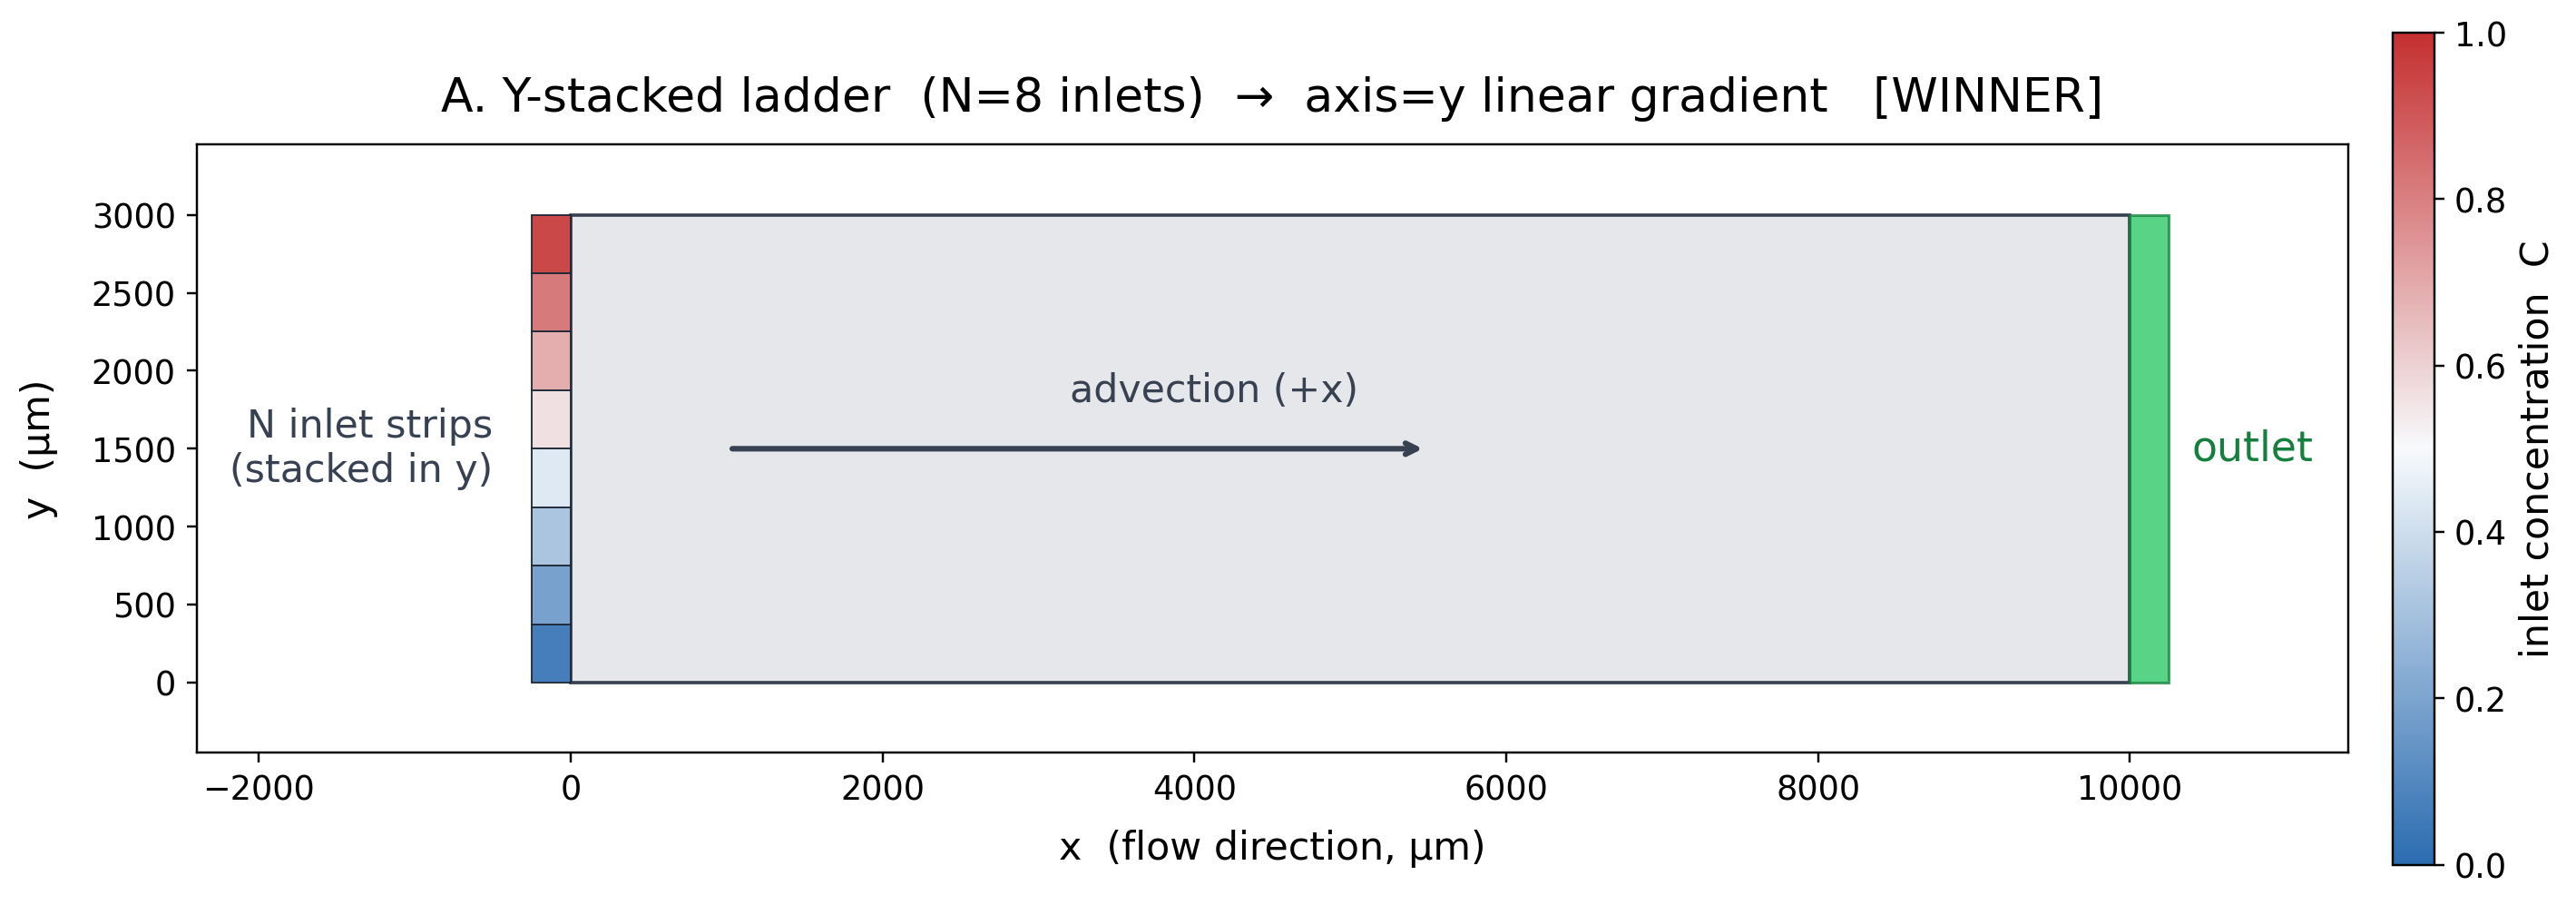
\includegraphics[width=0.6\textwidth]{A_ladder_N8 (1).png}\\[6pt]
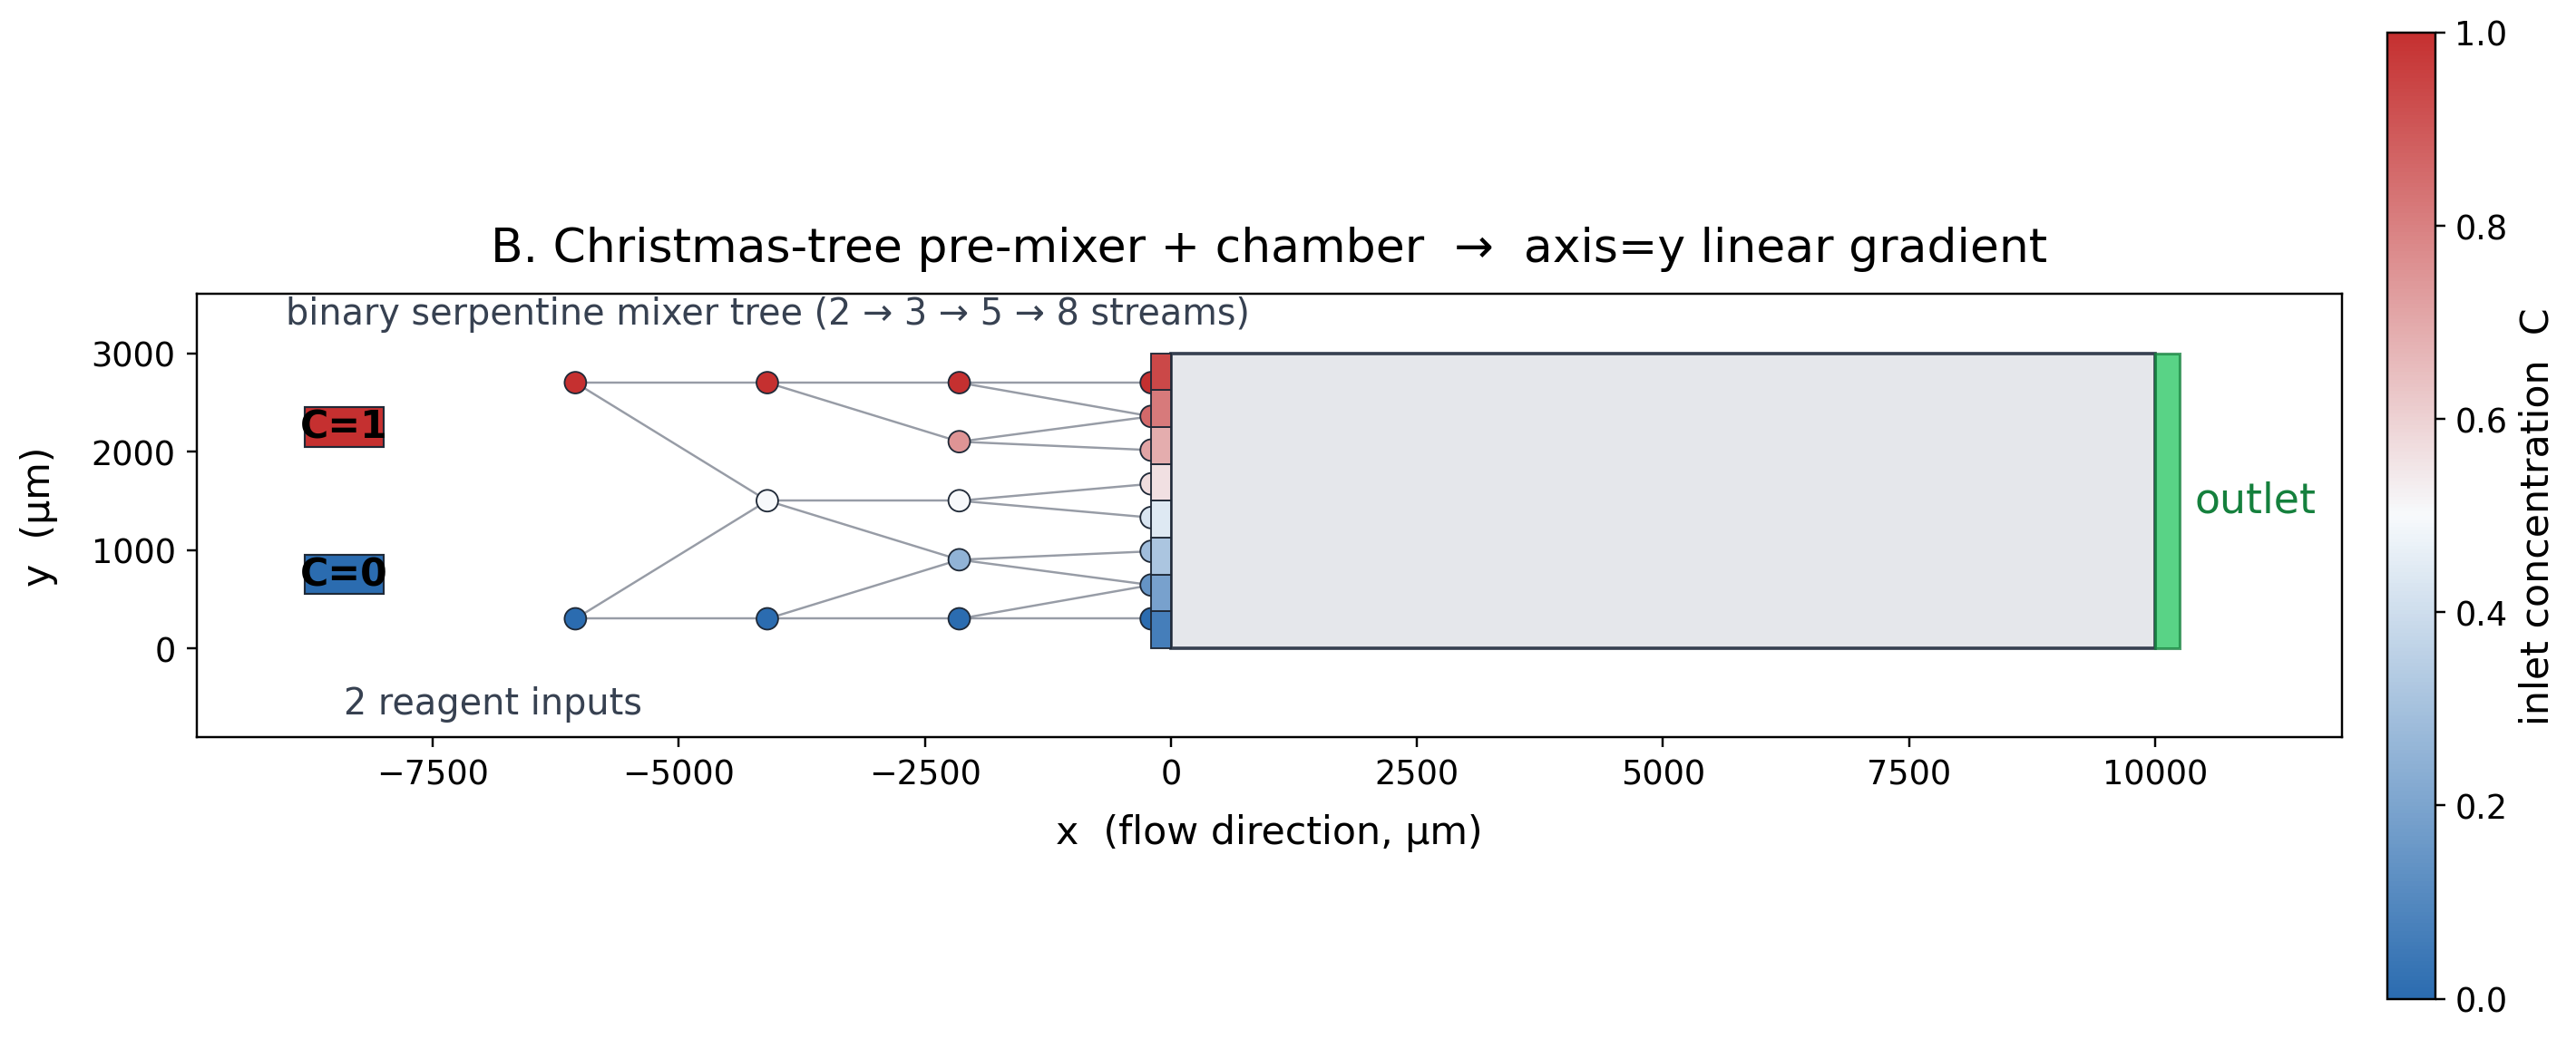
\includegraphics[width=0.6\textwidth]{B_christmas_tree.png}\\[6pt]
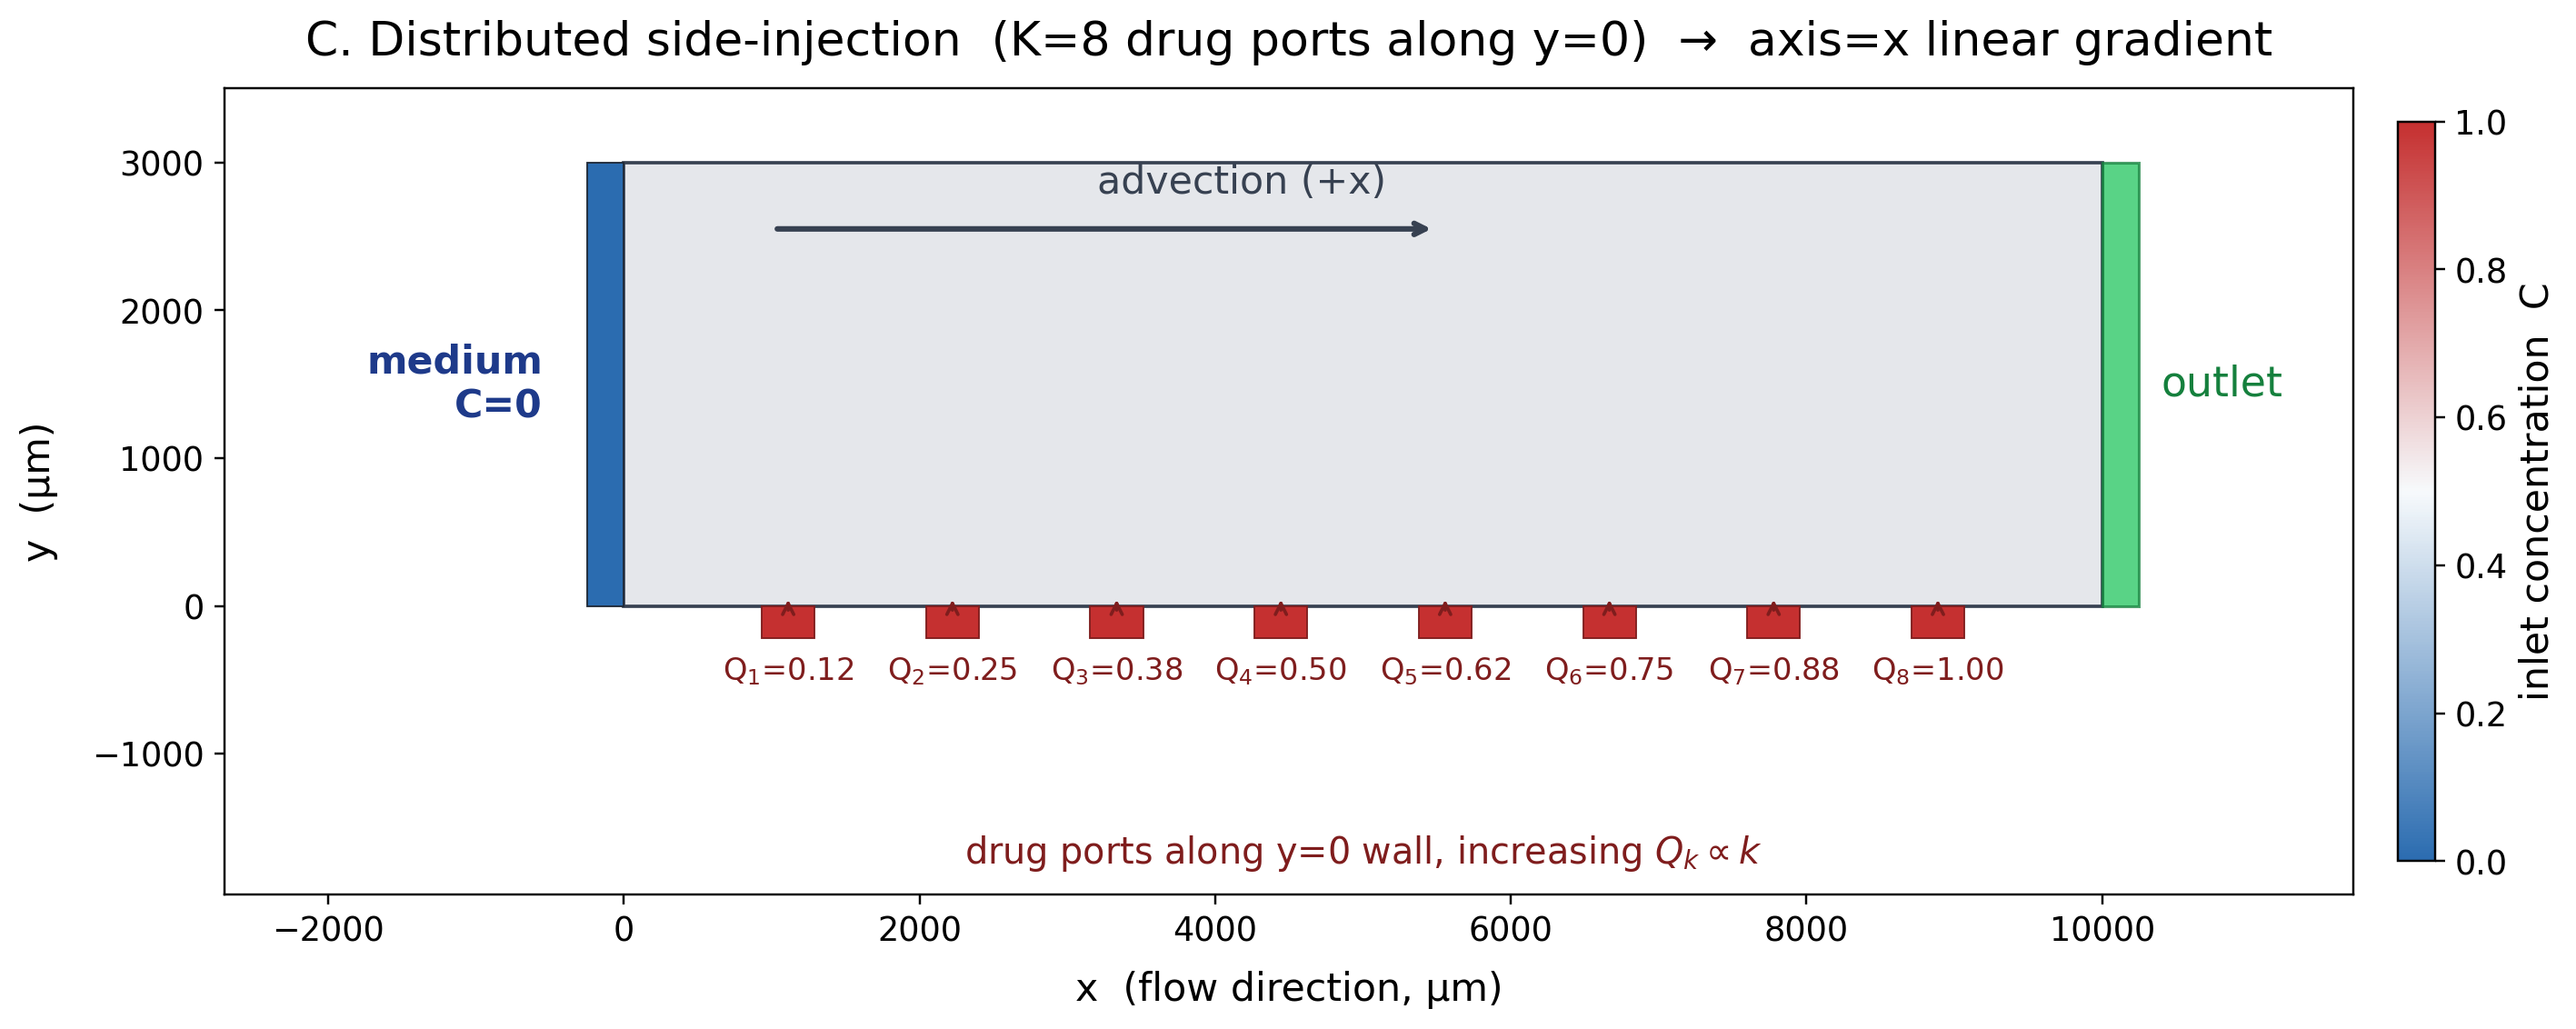
\includegraphics[width=0.6\textwidth]{C_side_injection_K8.png}\\[6pt]
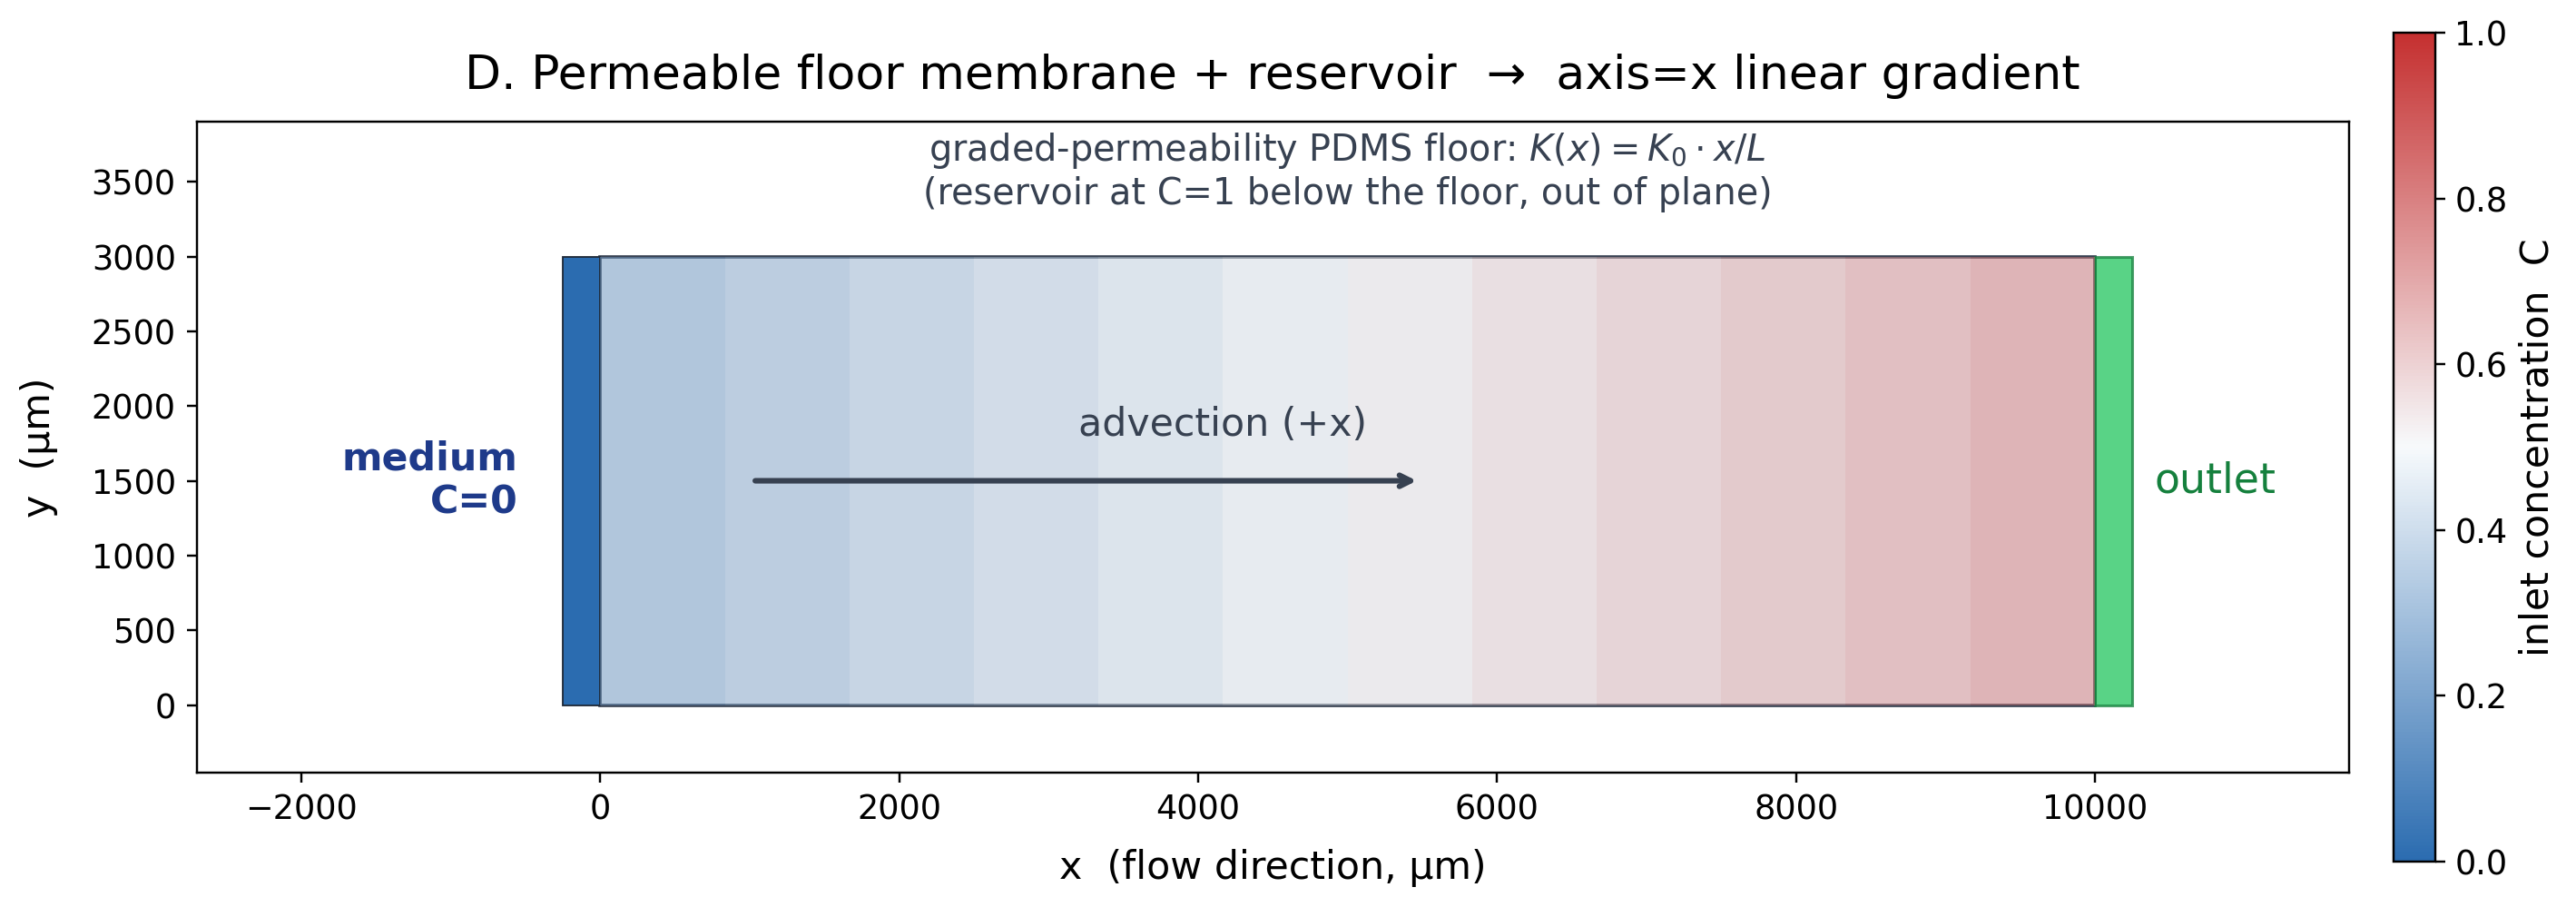
\includegraphics[width=0.6\textwidth]{D_permeable_wall.png}\\[6pt]
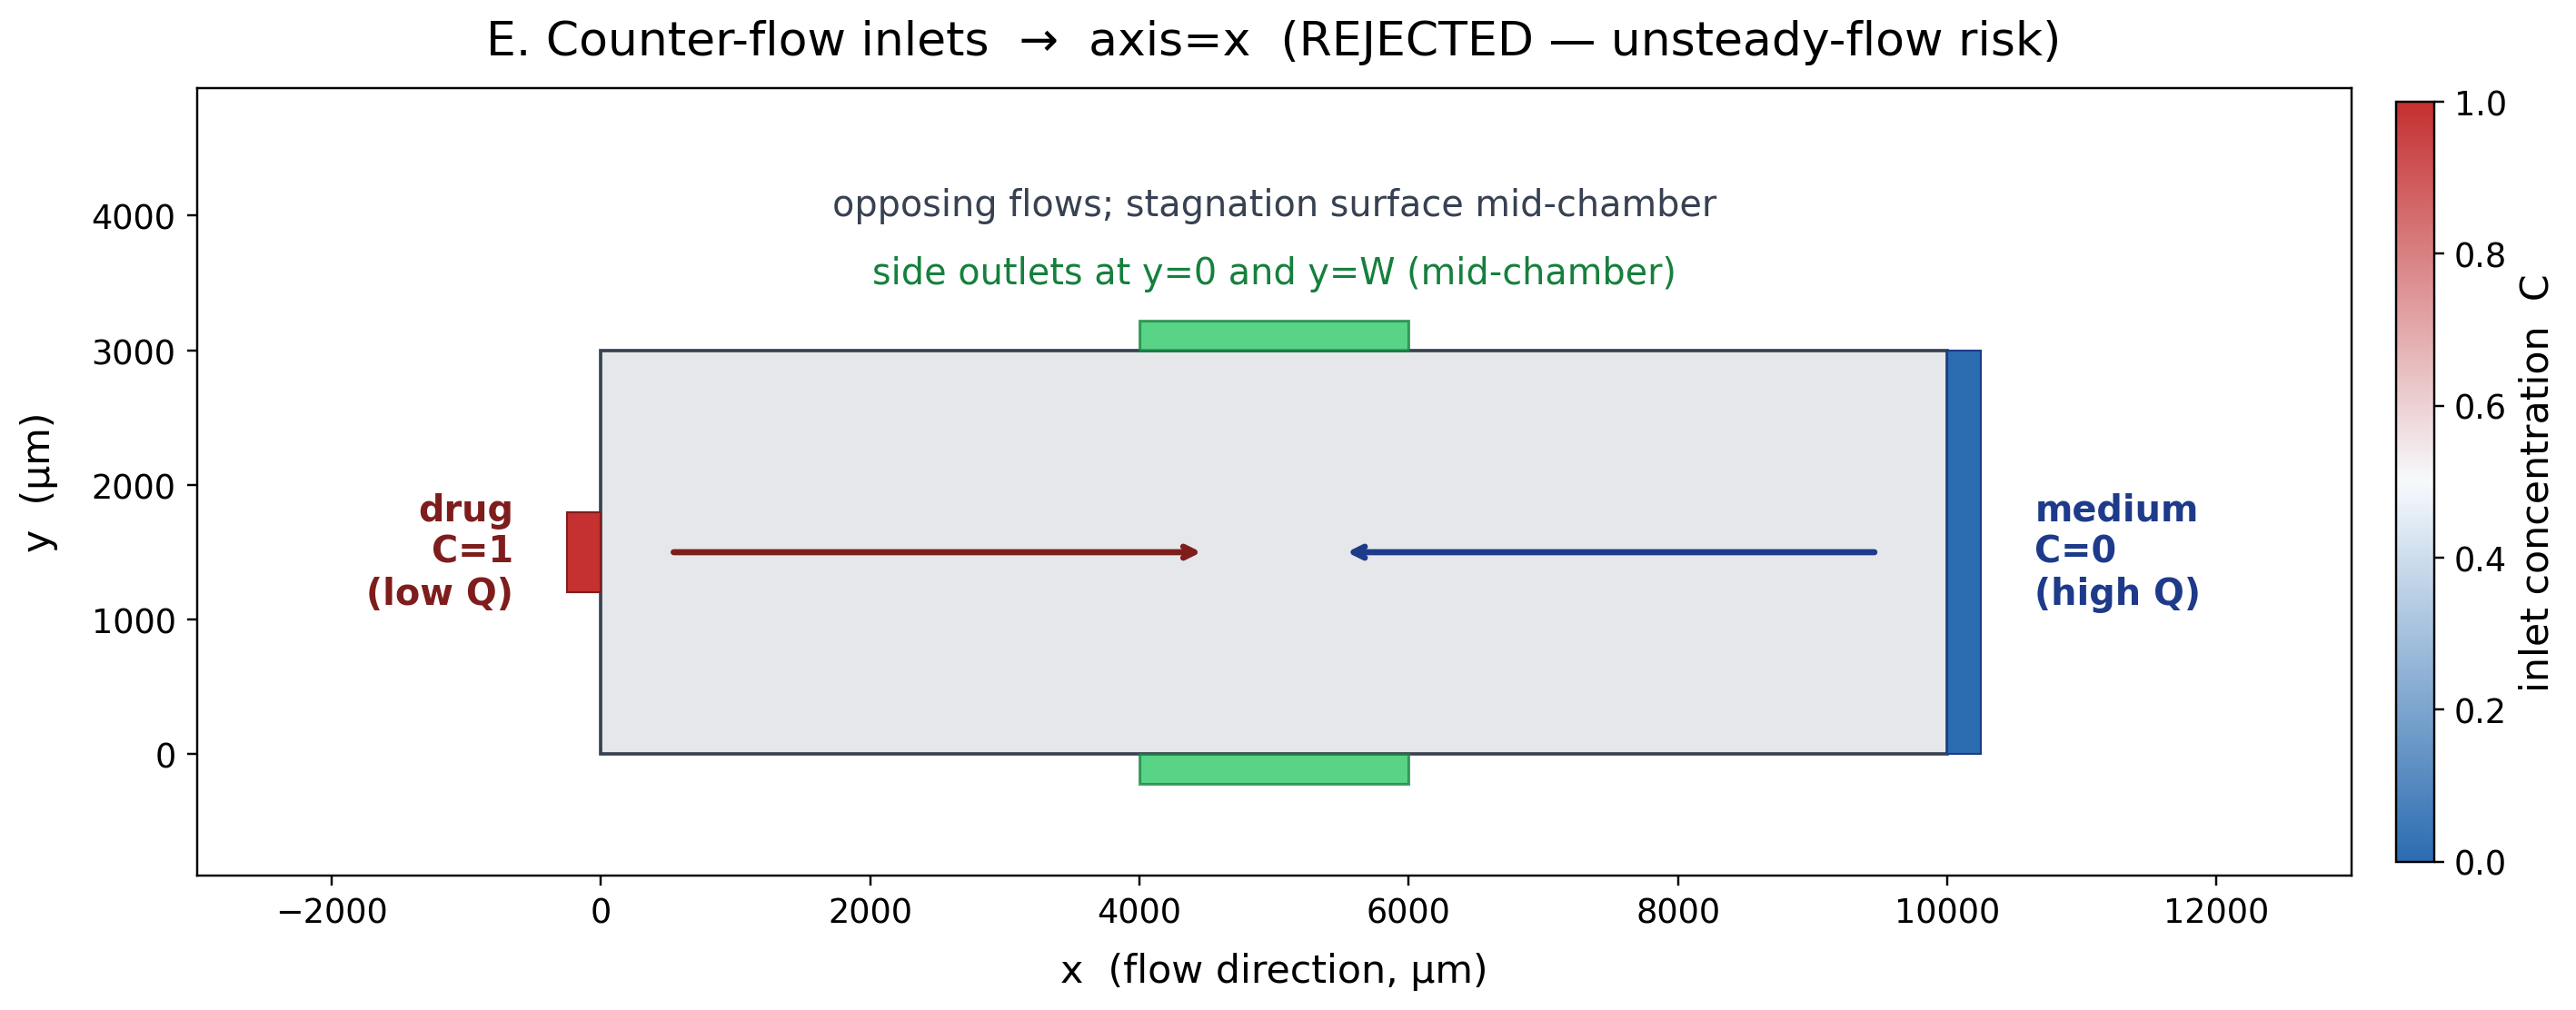
\includegraphics[width=0.6\textwidth]{E_counter_flow.png}
\caption{Schematic of the five Trial-2 candidate topologies (top to bottom): A.~stacked ladder, B.~Christmas-tree mixer, C.~distributed side injection, D.~permeable wall, E.~counter-flow. Only the ladder was implemented end-to-end in this study; the remaining four were ruled in or out by first-principles physical analysis (Section~\ref{sec:topology_screening}, Table~\ref{tab:admissibility}).}
\label{fig:topology_candidates}
\end{figure}

Single-shot CFD against the axis-$y$ target at fixed $H = 200~\mu$m, $W = 3000~\mu$m, $Q_{\text{total}} = 50~\mu$L/min produces the entries in Table~\ref{tab:ladder_single_shot}. The midpoint convention reduces $L_2$ by $38\%$ at $N = 8$, $L_2$ saturates by $N = 8$ (no further improvement at $N = 16$), and the observed $L_2 \approx 0.110$ sits at $1.76\times$ the analytical within-strip step-quantisation floor of $1/(2N\sqrt{3}) \cdot \sqrt{3} = 1/(2N) = 0.0625$. The remaining gap is dominated by upwind numerical diffusion at the production mesh (Section~\ref{sec:residual_budget}).

\begin{table}[H]
\centering
\caption{Single-shot ladder performance against the axis-$y$ linear gradient ($H = 200~\mu$m, $W = 3000~\mu$m, $Q_{\text{total}} = 50~\mu$L/min). The endpoint vs.\ midpoint comparison at fixed $N = 8$ is the source of the $38\%$ ``free'' improvement.}
\label{tab:ladder_single_shot}
\begin{tabular}{l c c}
\toprule
\textbf{Configuration} & $\boldsymbol{L_2}$ & \textbf{Improvement vs.\ baseline} \\
\midrule
Opposing winner (axis $= x$, reference) & 0.6343 & --- \\
Ladder $N = 4$, midpoint                 & 0.1337 & $4.7\times$ \\
Ladder $N = 8$, endpoint                 & 0.1756 & $3.6\times$ \\
Ladder $N = 8$, \textbf{midpoint}        & \textbf{0.1097} & $\boldsymbol{5.8\times}$ \\
Ladder $N = 16$, midpoint                & 0.1091 & $5.8\times$ (saturates) \\
\bottomrule
\end{tabular}
\end{table}

A 32-evaluation Sobol-quasirandom scan over $W \in [1500, 4500]~\mu$m and $Q_{\text{total}} \in [5, 200]~\mu$L/min ($N = 8$, \emph{endpoint convention}) returned $L_2 \in [0.1720, 0.1759]$---essentially flat (Figure~\ref{fig:phase2_scan}). The apparent contradiction between the flat scan and the $L_2 \approx 0.082$ achieved by the production BO is resolved entirely by the convention discrepancy: the scan used endpoint values, the production loop uses midpoint values, and the latter are uniformly $38\%$ better at any fixed geometry. The midpoint convention is now the production default.

\begin{figure}[H]
\centering
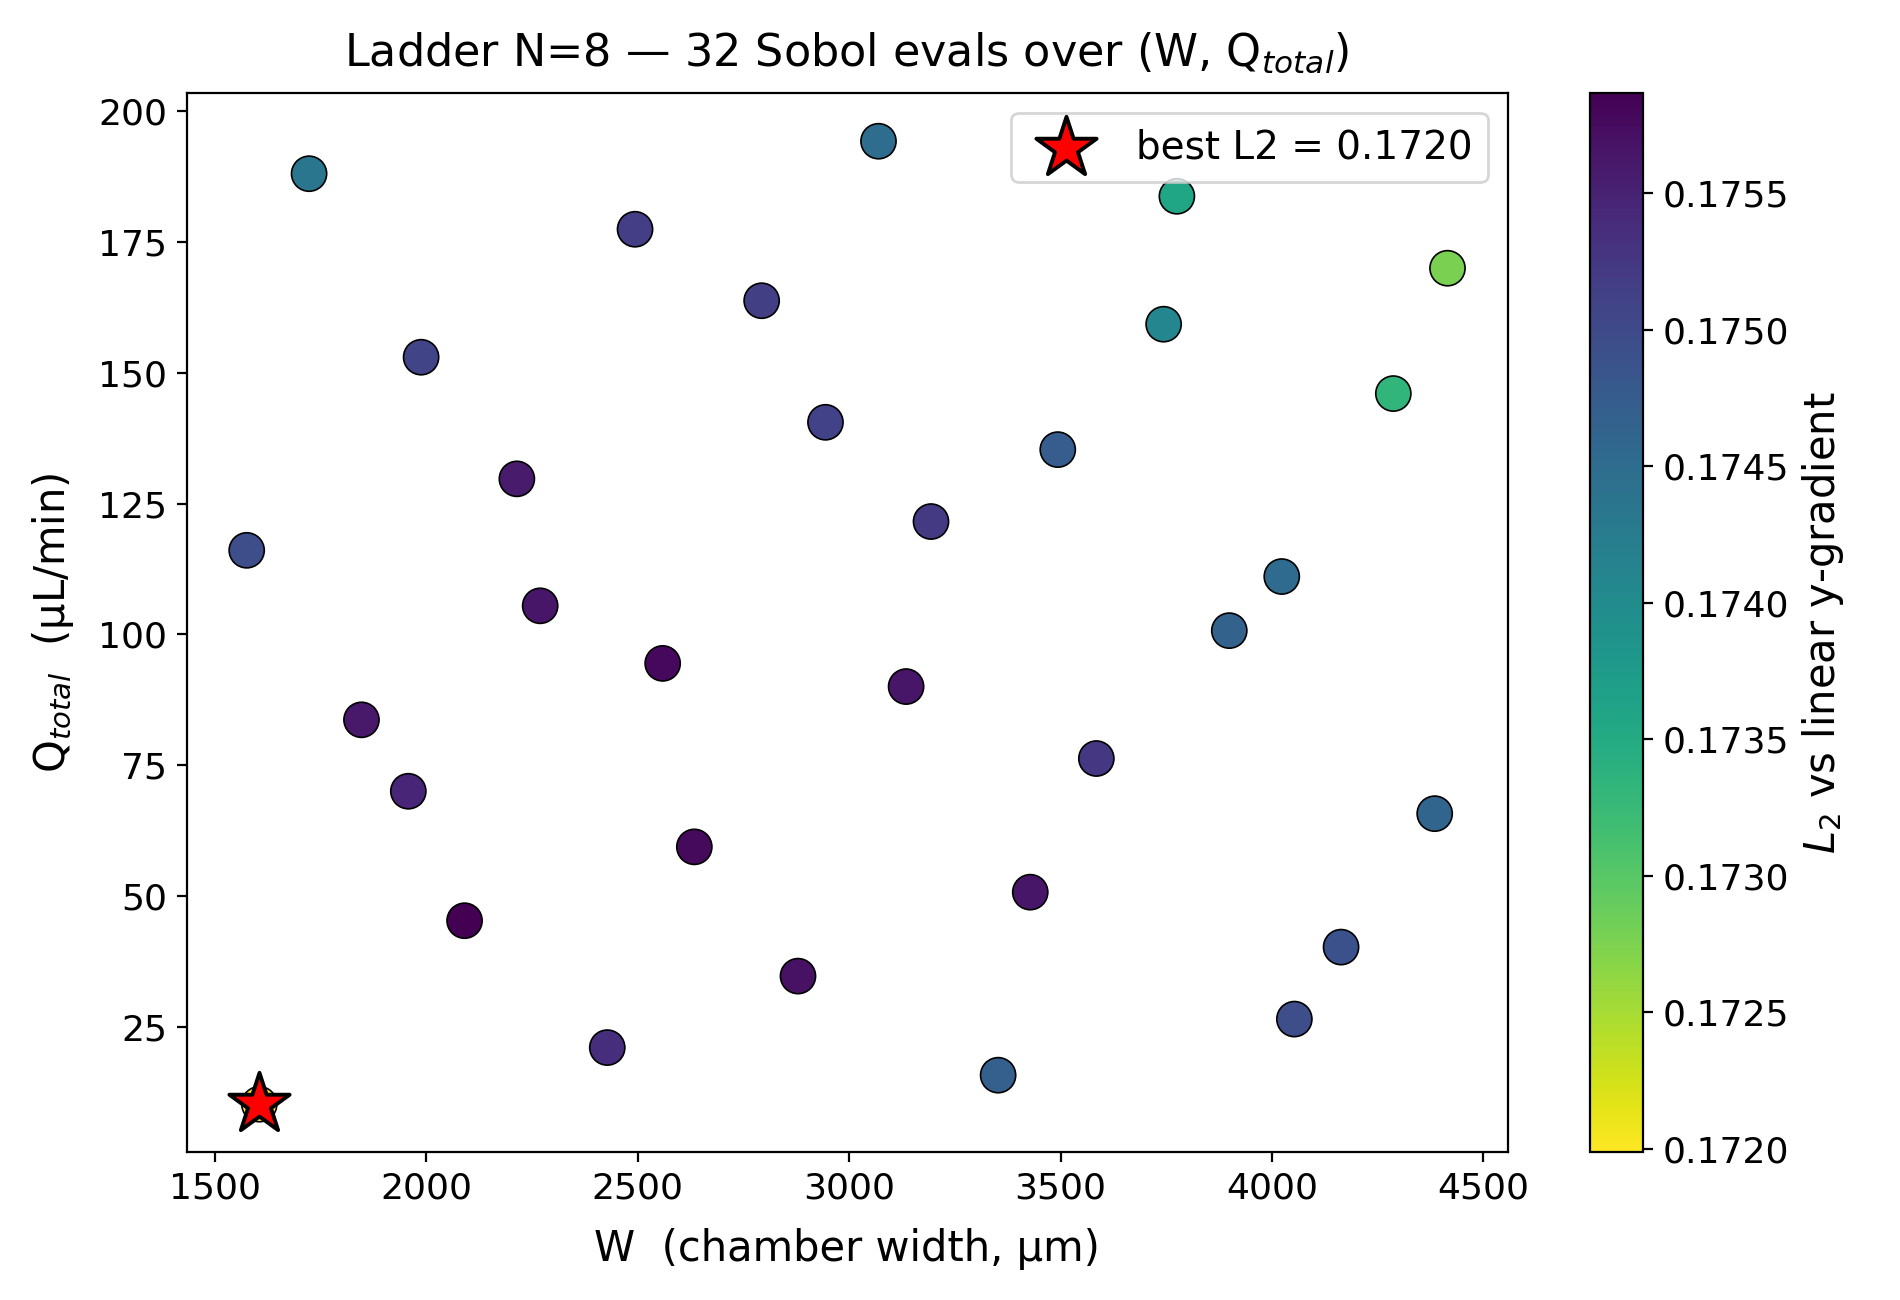
\includegraphics[width=0.65\textwidth]{phase2_W_Q_scan.png}
\caption{Sobol-quasirandom scan of the ladder topology over $W$ and $Q_{\text{total}}$ at $H = 200~\mu$m, using the \emph{endpoint} concentration convention (32 evaluations). $L_2$ values are confined to $[0.172, 0.176]$. The scan is flat because the imposed inlet pattern dominates the response; switching to the midpoint convention drops $L_2$ uniformly by $38\%$ to the $\sim 0.110$ regime of Table~\ref{tab:ladder_single_shot}, and full BO over $(W, Q_{\text{total}})$ reduces $L_2$ further to $0.082$ (Section~\ref{sec:bo_h200}).}
\label{fig:phase2_scan}
\end{figure}

\subsection{Cross-topology Bayesian Optimization at $H = 200~\mu$m}
\label{sec:bo_h200}
A 200-evaluation BO campaign per topology was run against the axis-$y$ linear-gradient target under the full five-constraint feasibility set (Table~\ref{tab:constraints}). Convergence trajectories appear in Figure~\ref{fig:bo_convergence}(a); the topology gap of roughly an order of magnitude is established within the Sobol initialisation (the first $24$ evaluations) and is preserved by the BO acquisition. Table~\ref{tab:cross_topology_summary} summarises the best-feasible $L_2$ and feasibility rates.

\begin{figure}[H]
\centering
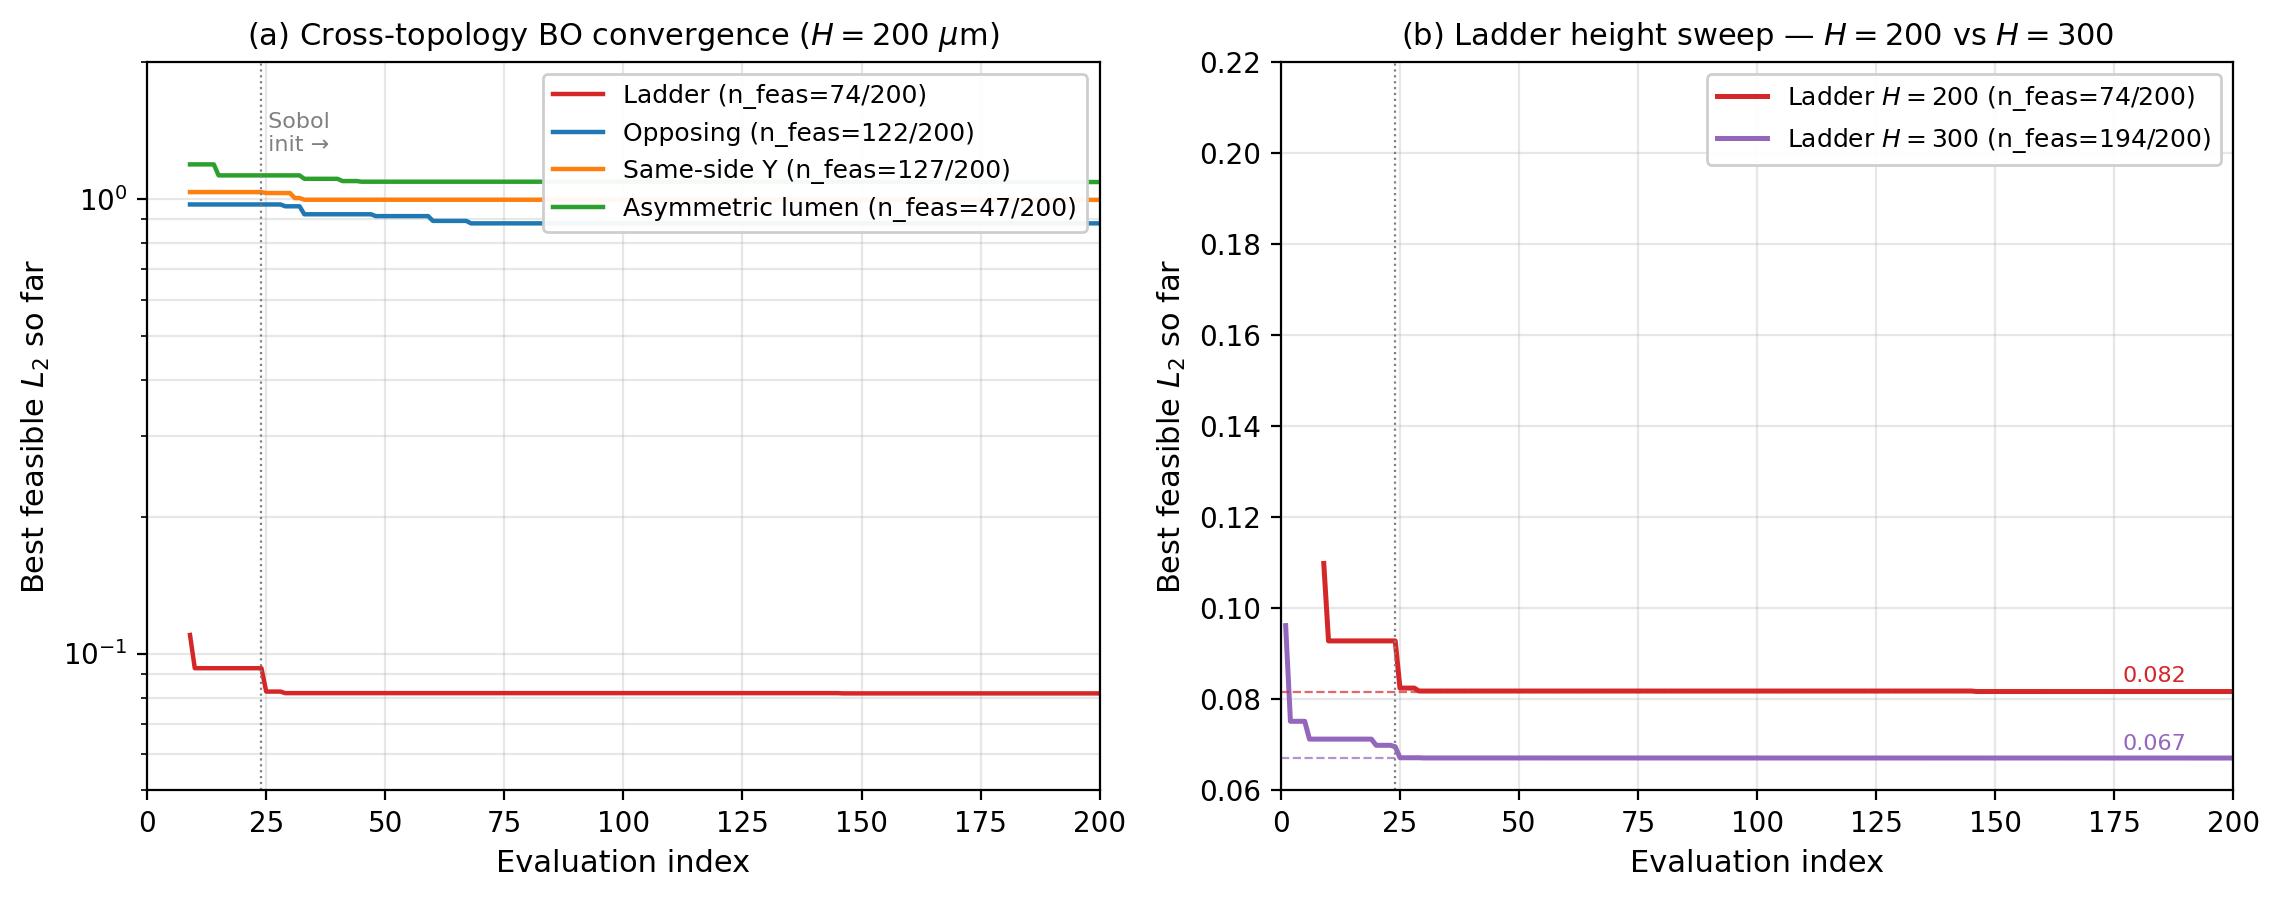
\includegraphics[width=0.95\textwidth]{fig_d_bo_convergence.png}
\caption{BO convergence curves. (a) All four topologies at $H = 200~\mu$m on a log-$y$ axis. The grey vertical line marks the Sobol-init / BO boundary at evaluation $24$. The ladder--two-inlet gap is established within the random initialisation; the BO acquisition refines the ladder optimum but does not change the topology ranking. (b) Ladder-only $H = 200$ vs $H = 300$ on a linear axis. Asymptotes drawn at $L_2 = 0.082$ ($H = 200$, red) and $L_2 = 0.067$ ($H = 300$, purple); $H = 300$ also raises feasibility from $74/200$ to $194/200$ over the same 200-evaluation budget.}
\label{fig:bo_convergence}
\end{figure}

\begin{table}[H]
\centering
\caption{Cross-topology BO summary at $H = 200~\mu$m, axis $= y$.}
\label{tab:cross_topology_summary}
\begin{tabular}{l c c c}
\toprule
\textbf{Topology} & \textbf{Best feasible $L_2$} & \textbf{Feasible / total} & \textbf{Active dims} \\
\midrule
\textbf{Ladder} (winner) & \textbf{0.0818} & $89/200$ ($44\%$) & 2 ($W, Q_{\text{total}}$) \\
Opposing                 & 0.8822          & $122/200$ ($61\%$) & 5 \\
Same-side Y              & 0.9937          & $127/200$ ($64\%$) & 4 \\
Asymmetric lumen         & 1.0875          & $47/200$  ($24\%$) & 4 \\
\bottomrule
\end{tabular}
\end{table}

The ladder beats the next-best topology by $10.8\times$ on the same axis-$y$ target: an apples-to-apples comparison under identical constraints, mesh, BO budget, and target. Numerically, the ladder winner reaches $L_2 = 0.0818$, $R^2_{\text{lin}} = 0.987$ at $W = 3000~\mu$m (the aspect ratio binding at $W/H = 15$) and $Q_{\text{total}} = 119.5~\mu$L/min, with $\tau_{\text{mean}} = 1.992$~Pa---within $0.1\%$ of the $2.0$~Pa cap. Both the aspect-ratio and shear-stress constraints are simultaneously active. The two-inlet topologies hover near the uniform-field $L_2$ floor for axis-$y$ ($\approx 1.0$ at $r_{\text{flow}} = 0.5$), confirming that the mass-conservation limit on streamwise linear gradients also bounds these topologies on transverse linear targets within the laminar regime sampled here.

\subsection{Extended Height Sweep: $H = 300~\mu$m Outperforms $H = 200~\mu$m}
\label{sec:h_sweep}
The $H = 200$ optimum sat at the intersection of two active constraints: aspect ratio ($W/H = 15$) and mean shear stress ($\tau_{\text{mean}} = 1.998$~Pa, within $0.1\%$ of the $2.0$~Pa cap), with a feasibility rate of $37.0\%$. Dimensional analysis predicts $\tau \propto Q / (W H^2)$, so opening $H$ from $200$ to $300~\mu$m provides $\sim 2.25\times$ more shear-stress headroom at fixed $(W, Q)$. The ladder BO was therefore re-run at $H = 300~\mu$m with all other settings unchanged. Table~\ref{tab:h_sweep} compares the results; convergence appears in Figure~\ref{fig:bo_convergence}(b).

\begin{table}[H]
\centering
\caption{Ladder performance at $H = 200$ vs $H = 300~\mu$m. Both campaigns used the same configuration except for chamber height.}
\label{tab:h_sweep}
\begin{tabular}{l c c}
\toprule
\textbf{Quantity} & $\boldsymbol{H = 200~\mu\text{m}}$ & $\boldsymbol{H = 300~\mu\text{m}}$ \\
\midrule
Best feasible $L_2$         & 0.0817 & \textbf{0.0671} \\
Best $W$ ($\mu$m)           & 2999 (cap) & \textbf{4496 (cap)} \\
Best $Q_{\text{total}}$ ($\mu$L/min) & 119.8 & \textbf{200.0 (cap)} \\
$\tau_{\text{mean}}$ (Pa)   & \textbf{1.998 (cap)} & 1.483 \\
Aspect ratio $W/H$          & \textbf{15.00 (cap)} & \textbf{14.99 (cap)} \\
Re                          & 24.97 & 41.71 \\
$R^2$-to-linear             & 0.987 & \textbf{0.990} \\
$C_{\text{std}}$            & 0.314 & 0.306 \\
Feasibility rate            & 37.0\% & \textbf{96.5\%} \\
\bottomrule
\end{tabular}
\end{table}

Opening $H$ from $200$ to $300~\mu$m reduces $L_2$ by $17.9\%$, matching the dimensional-analysis pre-test prediction of $\sim 0.069$ within $2\%$. The constraint corner shifts: aspect ratio still binds ($W \approx 4500~\mu$m), but $\tau_{\text{mean}}$ releases ($1.48 \ll 2.0$~Pa) and $Q_{\text{total}}$ saturates at its $200~\mu$L/min upper bound (a configuration choice rather than a physical limit; typical syringe pumps deliver up to $\sim 1000~\mu$L/min). The slight gap of $W = 4496$ from $4500$ reflects the bisection-tolerance precision of the BO acquisition near the corner; at $H = 300$ the $W$ cap and the $W/H \leq 15$ cap are degenerate. Feasibility nearly triples, from $37.0\%$ to $96.5\%$, so the $H = 300$ surrogate is fitted on $\sim 2.6\times$ more useful data and is correspondingly more reliable for downstream interpretability.

Figure~\ref{fig:concentration_field} shows the converged concentration field of the $H = 300$ winner. The depth-averaged $\langle C \rangle_x(y)$ tracks the linear target at $R^2 = 0.990$. Three downstream stations at $x \in \{1, 5, 9\}$~mm reveal a transit length: at $x = 1$~mm the staircase shoulders from the imposed inlet ladder are still pronounced; by $x = 5$~mm the field has converged to within $\sim 1\%$ of the depth-averaged profile, and the $x = 5$~mm and $x = 9$~mm stations lie almost on top of each other. The chamber is therefore effectively a two-stage device---an inlet rounding region of $\sim 2$~mm where cross-stream diffusion smooths the strip steps, followed by an $\sim 8$~mm steady-gradient region.

\begin{figure}[H]
\centering
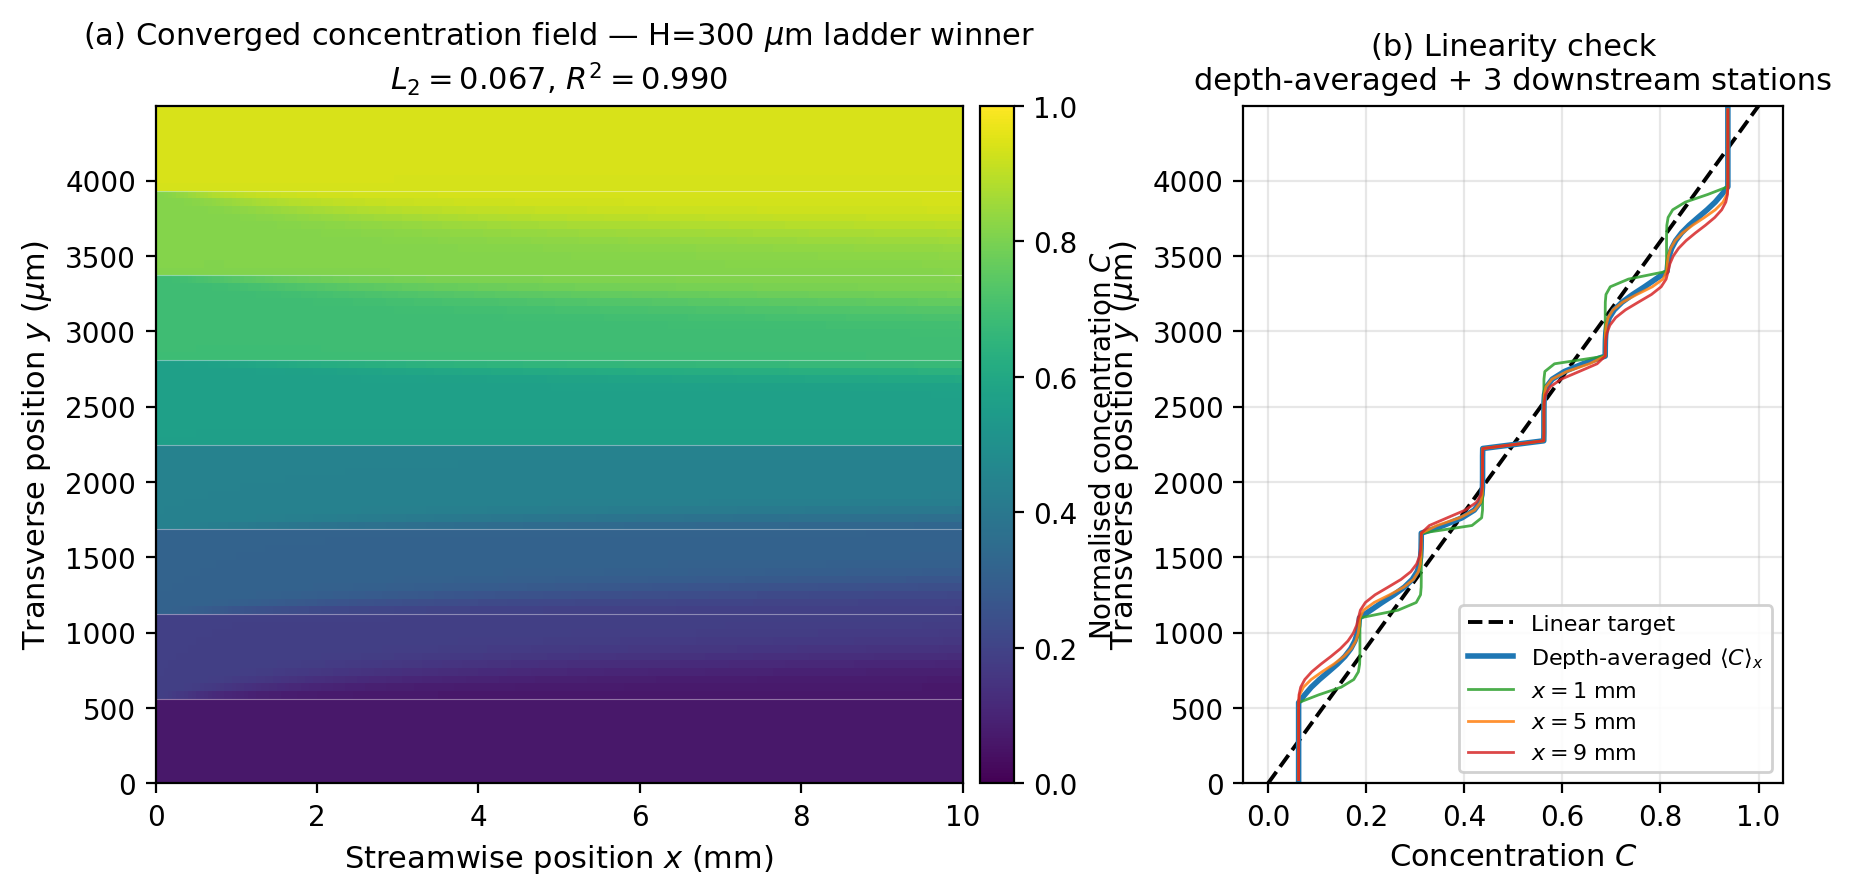
\includegraphics[width=0.95\textwidth]{fig_e_concentration_field.png}
\caption{Converged concentration field of the $H = 300$ ladder winner ($L_2 = 0.067$, $R^2_{\text{lin}} = 0.990$). (a) 2-D normalised concentration $C(x, y)$ across the chamber; horizontal lines mark inlet-strip boundaries. (b) Depth-averaged $\langle C \rangle_x(y)$ profile (blue) overlaid on the linear target (dashed black) and three downstream-station profiles. The transit length over which the imposed staircase smooths to the linear target is $\sim 2$~mm.}
\label{fig:concentration_field}
\end{figure}

\subsection{Constraint-Binding Diagnostic and the Corner Shift}
The constraint-binding diagnostic at each topology's best-feasible design (Figure~\ref{fig:constraint_binding}) makes the $H = 200 \to H = 300$ corner shift visually unambiguous. At $H = 200$ the ladder is pinned simultaneously on $W/H$ and $\tau_{\text{mean}}$; at $H = 300$ the pinning pair becomes $W/H$ and $Q_{\text{total}}$, with $\tau_{\text{mean}}$ released. Same-side Y and asymmetric lumen are both pinned on $\tau_{\text{mean}}$ at their best-feasible designs at $H = 200$, plus $f_{\text{dead}}$ for asymmetric lumen (a topology-intrinsic stagnant-corner limitation). Reading off which constraints bind tells the experimentalist exactly which lab-side capability would most cheaply move the optimum---arguably the most actionable artefact of the pipeline.

\begin{figure}[H]
\centering
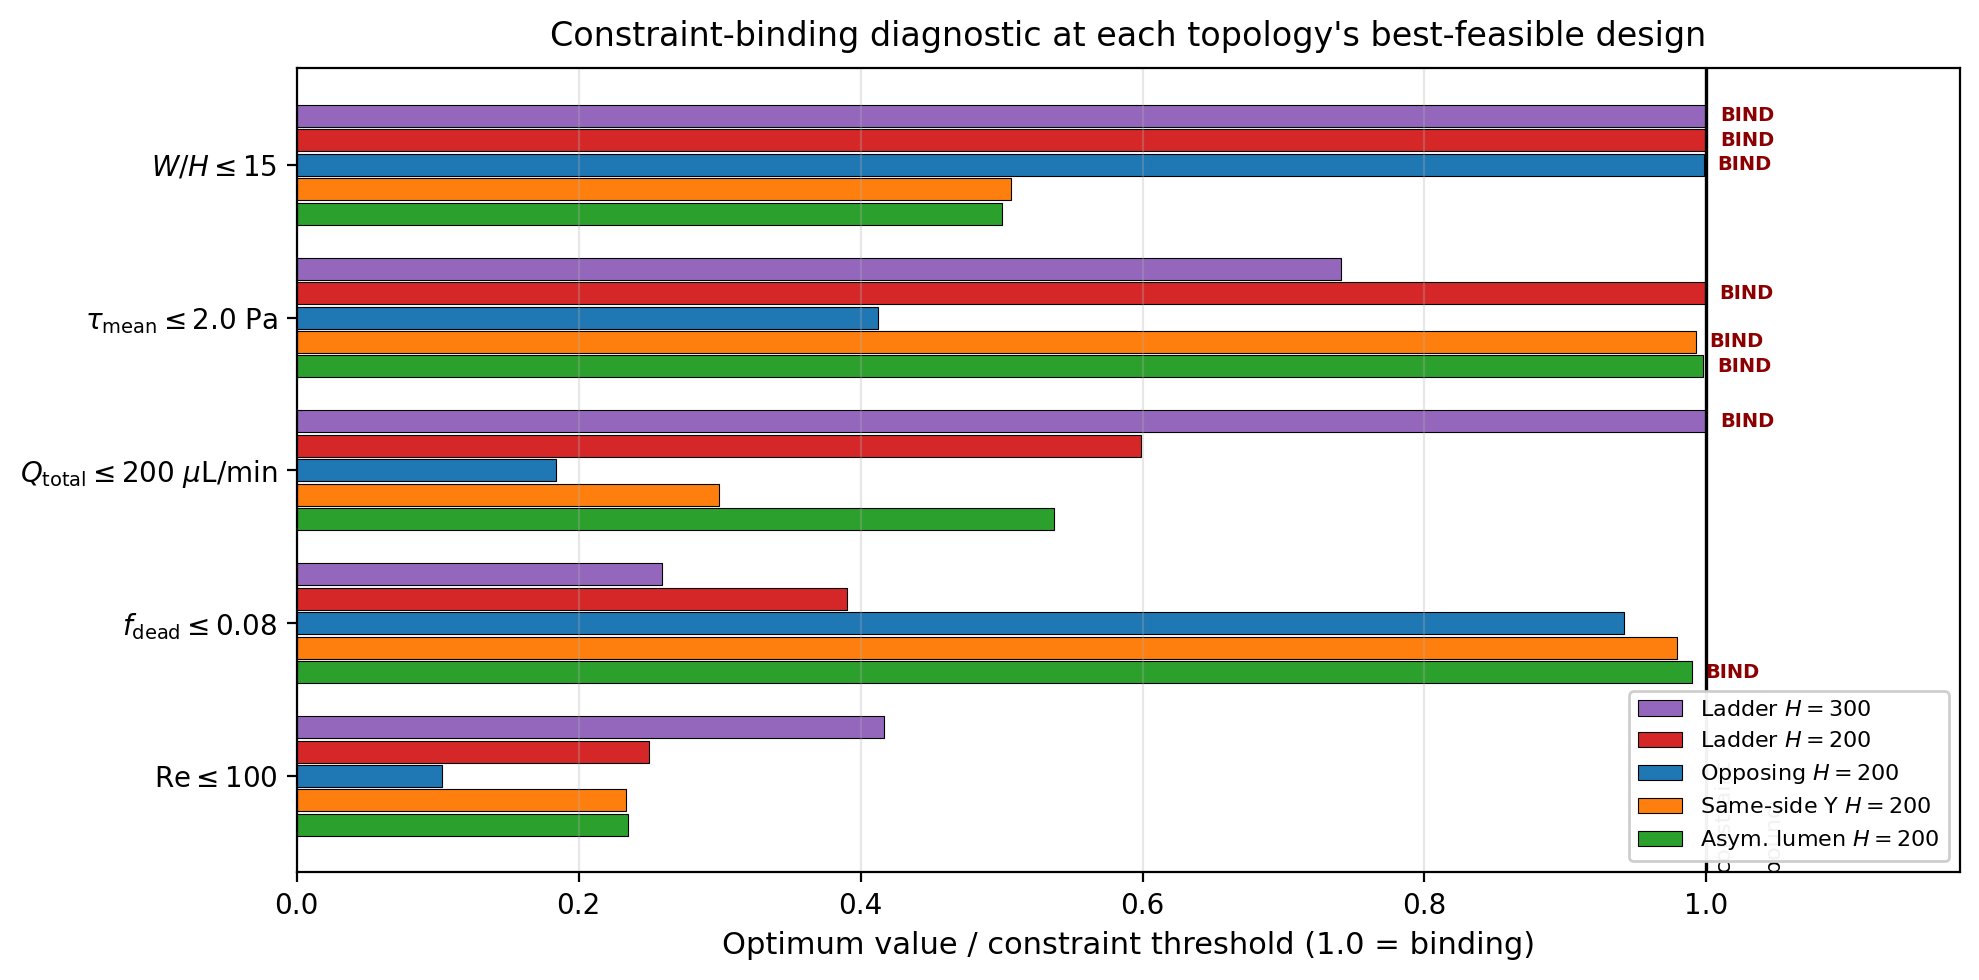
\includegraphics[width=0.95\textwidth]{fig_b_constraint_binding.png}
\caption{Constraint-binding diagnostic at each topology's best-feasible design. Bars show the optimum's value divided by the constraint threshold ($1.0 = $~binding; ``BIND'' annotated). The black vertical line at $1.0$ marks the constraint surface. Reading top-to-bottom for ladder $H = 300$: $W/H$ binds, $\tau_{\text{mean}}$ slack ($0.74$), $Q_{\text{total}}$ binds. The ladder $H = 200$ pair is ($W/H$, $\tau_{\text{mean}}$); the $H = 300$ pair becomes ($W/H$, $Q_{\text{total}}$).}
\label{fig:constraint_binding}
\end{figure}

\subsection{Cross-topology Sobol Interpretability: F1, F2, F3}
\label{sec:sobol}
Because the bare-ladder optimisation is 2-D in $(W, Q_{\text{total}})$ by construction, the cross-topology interpretability \emph{narrative} concentrates on the four-active-dim two-inlet topologies, where the GP surrogate has more dimensional structure to expose. Three findings recur across all three two-inlet topologies and survive the trustworthiness audit (Section~\ref{sec:audit}):
\begin{description}
\item[F1.] $r_{\text{flow}}$ is the universal driver. $S_T(r_{\text{flow}}) = 0.65$ (opposing, with overfit caveat), $0.86$ (same-side Y), $0.98$ (asymmetric lumen). The local-sensitivity rankings concur. Mechanistically, $r_{\text{flow}}$ is the only knob that moves the lateral position of the drug--medium interface---the sole structural feature these topologies can produce.
\item[F2.] $\theta$ (inlet convergence angle) is consistently inactive. $S_T(\theta) \approx 1.8 \times 10^{-4}$ (opposing), $1.6 \times 10^{-3}$ (same-side Y), $3.5 \times 10^{-5}$ (asymmetric lumen)---floor noise everywhere. Future studies can fix $\theta$ at its midpoint and save a dimension.
\item[F3.] $W$ and $Q_{\text{total}}$ trade off as the secondary lever. Same-side Y favours $W$ ($S_T = 0.13$) over $Q_{\text{total}}$ ($0.08$); asymmetric lumen reverses the ordering ($Q_{\text{total}} = 0.03 > W = 0.01$); opposing has both at low magnitudes (with caveat). The mechanism is direct: once $r_{\text{flow}}$ has placed the interface, the residual $L_2$ reduction comes from chamber width (more diffusion length) \emph{or} flow rate (higher Pe), whichever happens to be unconstrained; the two are interchangeable substitutes.
\end{description}

\begin{figure}[H]
\centering
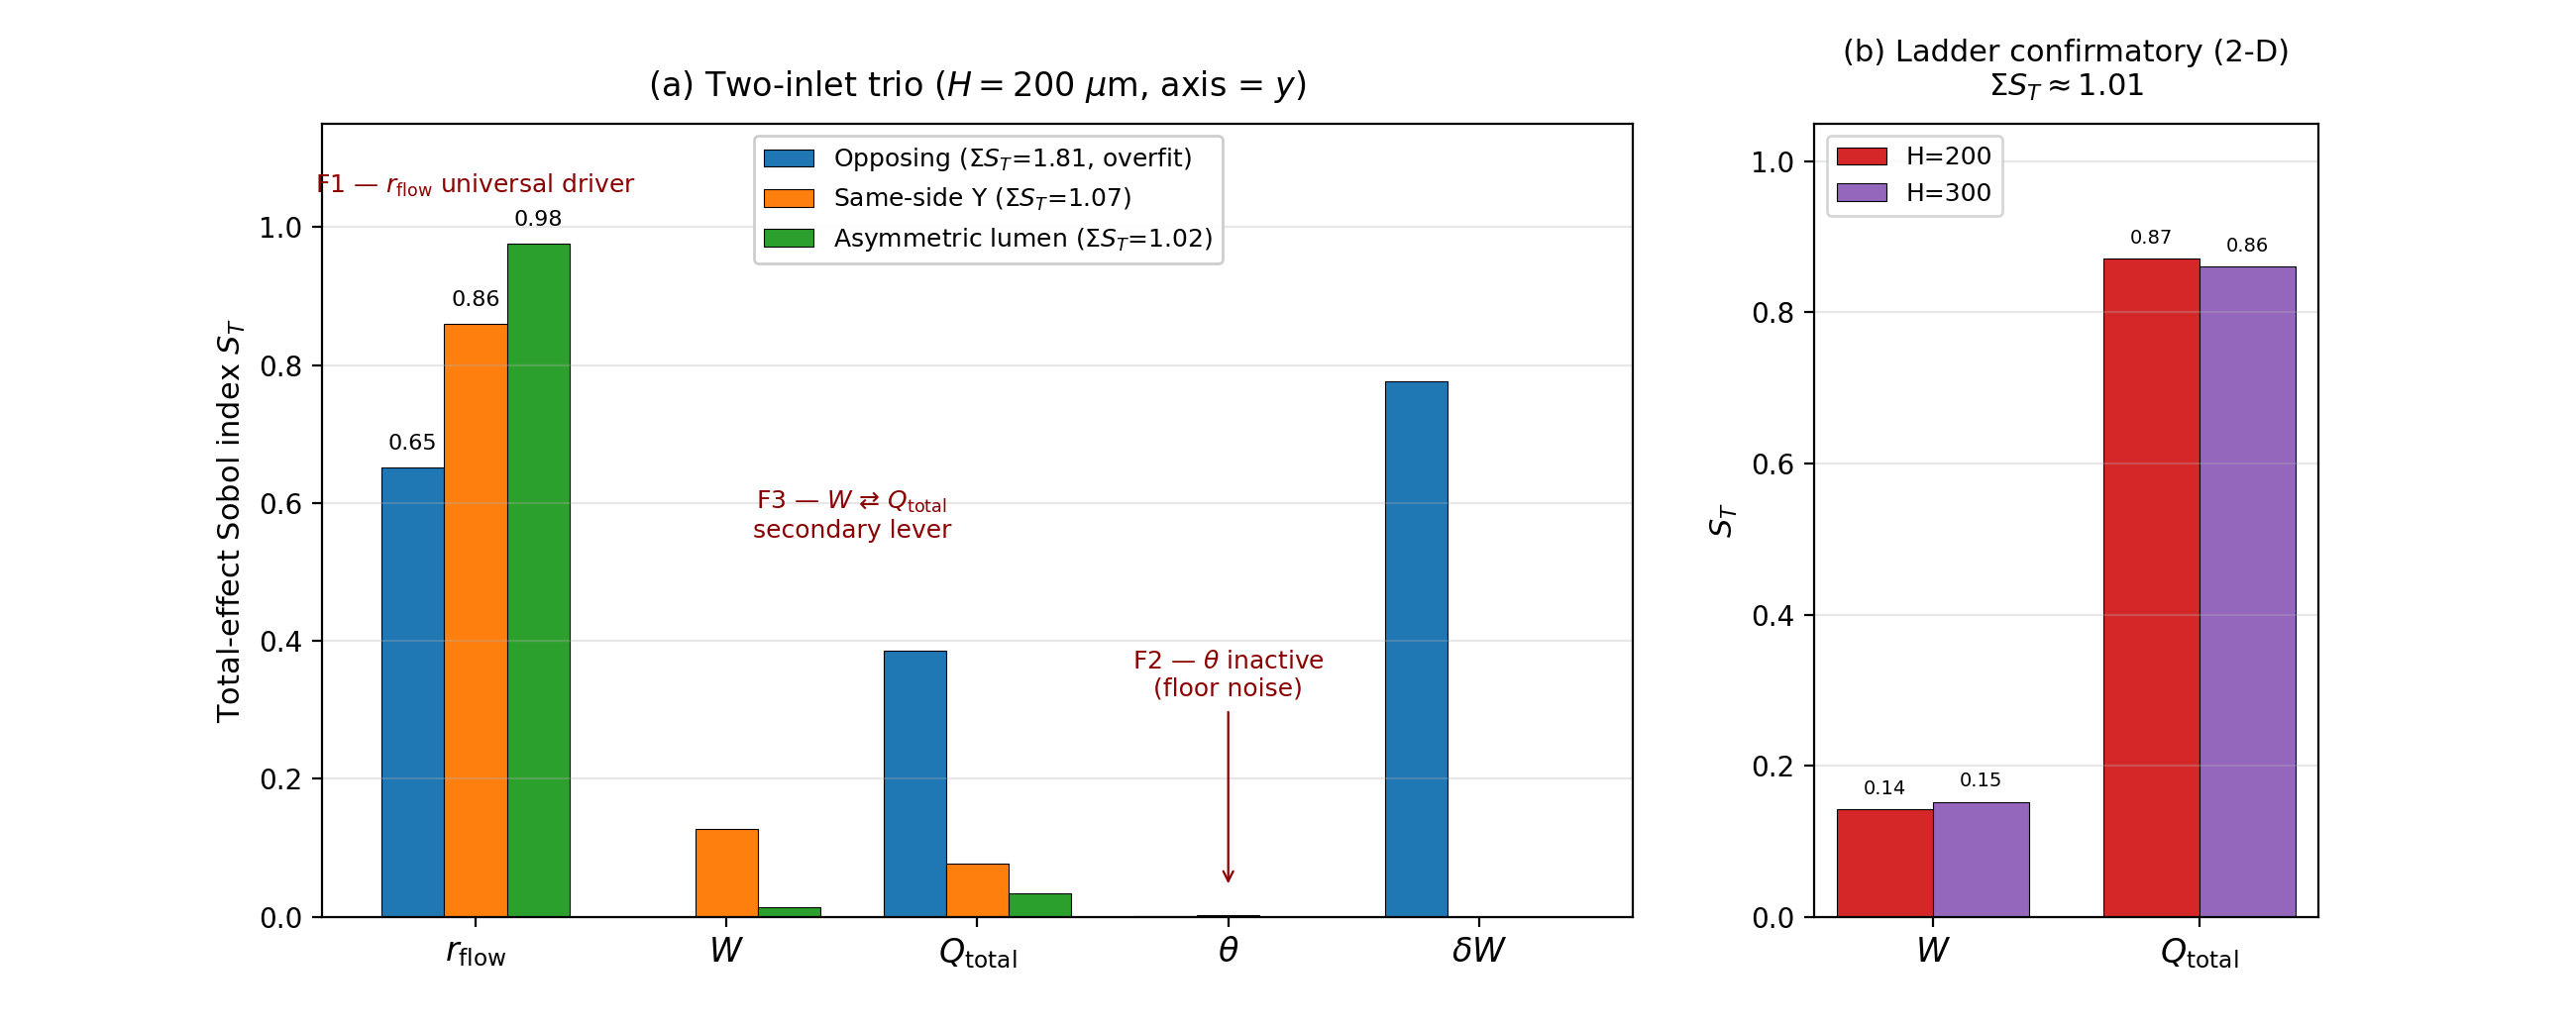
\includegraphics[width=0.99\textwidth]{fig_c_cross_topology_sobol.png}
\caption{Cross-topology Sobol total-effect indices. (a) Two-inlet trio at $H = 200~\mu$m, axis $= y$, with F1/F2/F3 spotlight annotations. The opposing topology is flagged $\Sigma S_T = 1.81$ (overfit; magnitudes inflated). (b) Confirmatory ladder Sobol at $H = 200$ and $H = 300$ over the active 2-D space ($W, Q_{\text{total}}$); both $\Sigma S_T \approx 1.01$.}
\label{fig:sobol}
\end{figure}

The ladder-confirmatory Sobol (Figure~\ref{fig:sobol}(b)) is consistent: $Q_{\text{total}}$ carries $\sim 0.87$ of $S_T$ at both heights, $W$ carries $\sim 0.14$--$0.15$. The slight rise of $W$'s share at $H = 300$ reflects the relaxed aspect-ratio cap that gives the BO more genuine search room in $W$. The flow-knob (ladder) versus interface-knob (two-inlet) dichotomy is a clean design heuristic: a topology with $\geq 3$ imposed-concentration inlets encodes the gradient directly into the boundary condition and the chamber's job is to advect that pattern without smearing, whereas a two-inlet coflow generates the gradient at the stream interface and the chamber's job is to position that interface. Section~\ref{sec:pillar_ablation} adds a third regime to this story.

\subsection{Pillar Ablation Reveals a Regime Swap}
\label{sec:pillar_ablation}
The original ladder optimisation masked five of seven design parameters under an a-priori assumption that ``only $W$ and $Q_{\text{total}}$ influence the field''. We tested this assumption empirically by unmasking the pillar diameter $d_p$ and pillar spacing $s_p$ via $\text{pillar\_config} = 1\!\times\!4$ and re-running a 100-evaluation constrained BO at $H = 200~\mu$m. The active design space becomes 4-D in $(W, d_p, s_p, Q_{\text{total}})$; the inlet-junction parameters ($\theta, r_{\text{flow}}, \delta_W$) remain structurally inactive for the ladder geometry generator and are still masked.

The result overturns the a-priori assumption in two ways. First, the best $L_2$ falls to $0.0568$ (a $\sim 30\%$ drop relative to the bare-ladder $H = 200$ winner of $0.0818$) at $W = 2121~\mu$m, $d_p = 184~\mu$m, $s_p = 427~\mu$m, $Q_{\text{total}} = 125~\mu$L/min, with $R^2_{\text{lin}} = 0.992$ and $\text{Re} = 31.9$ (laminar). Reported alongside the production constraint set, this design narrowly violates the $\tau_{\text{mean}} \leq 2.0$~Pa cap ($\tau = 2.62$~Pa); the best fully-feasible design under all five production constraints sits at $L_2 = 0.0588$, comparable to, but still below, the bare-ladder $H = 200$ winner---and well above the $H = 300$ winner of $0.067$, so the pillar gain is not yet fully captured under the production constraint set. Second, and more strikingly, the Sobol indices on the new 4-D surrogate \emph{invert} which knob controls the gradient (Figure~\ref{fig:pillar_swap}, Table~\ref{tab:pillar_sobol}).

\begin{table}[H]
\centering
\caption{Sobol total-effect indices for the ladder topology under the two pillar configurations. The bare-ladder run is the $H = 200$ entry from Section~\ref{sec:sobol}; the pillar run is the new ablation at $H = 200$, $\text{pillar\_config} = 1\!\times\!4$. ``masked'' indicates the parameter was not optimised in that run.}
\label{tab:pillar_sobol}
\begin{tabular}{l c c}
\toprule
\textbf{Parameter} & $\boldsymbol{S_T}$ \textbf{(pillars = none)} & $\boldsymbol{S_T}$ \textbf{(pillars = 1$\times$4)} \\
\midrule
$W$               & $0.143$ & $\mathbf{0.856}$ \\
$Q_{\text{total}}$& $\mathbf{0.871}$ & $0.001$ \\
$s_p$             & masked & $\mathbf{0.139}$ \\
$d_p$             & masked & $0.009$ \\
\bottomrule
\end{tabular}
\end{table}

\begin{figure}[H]
\centering
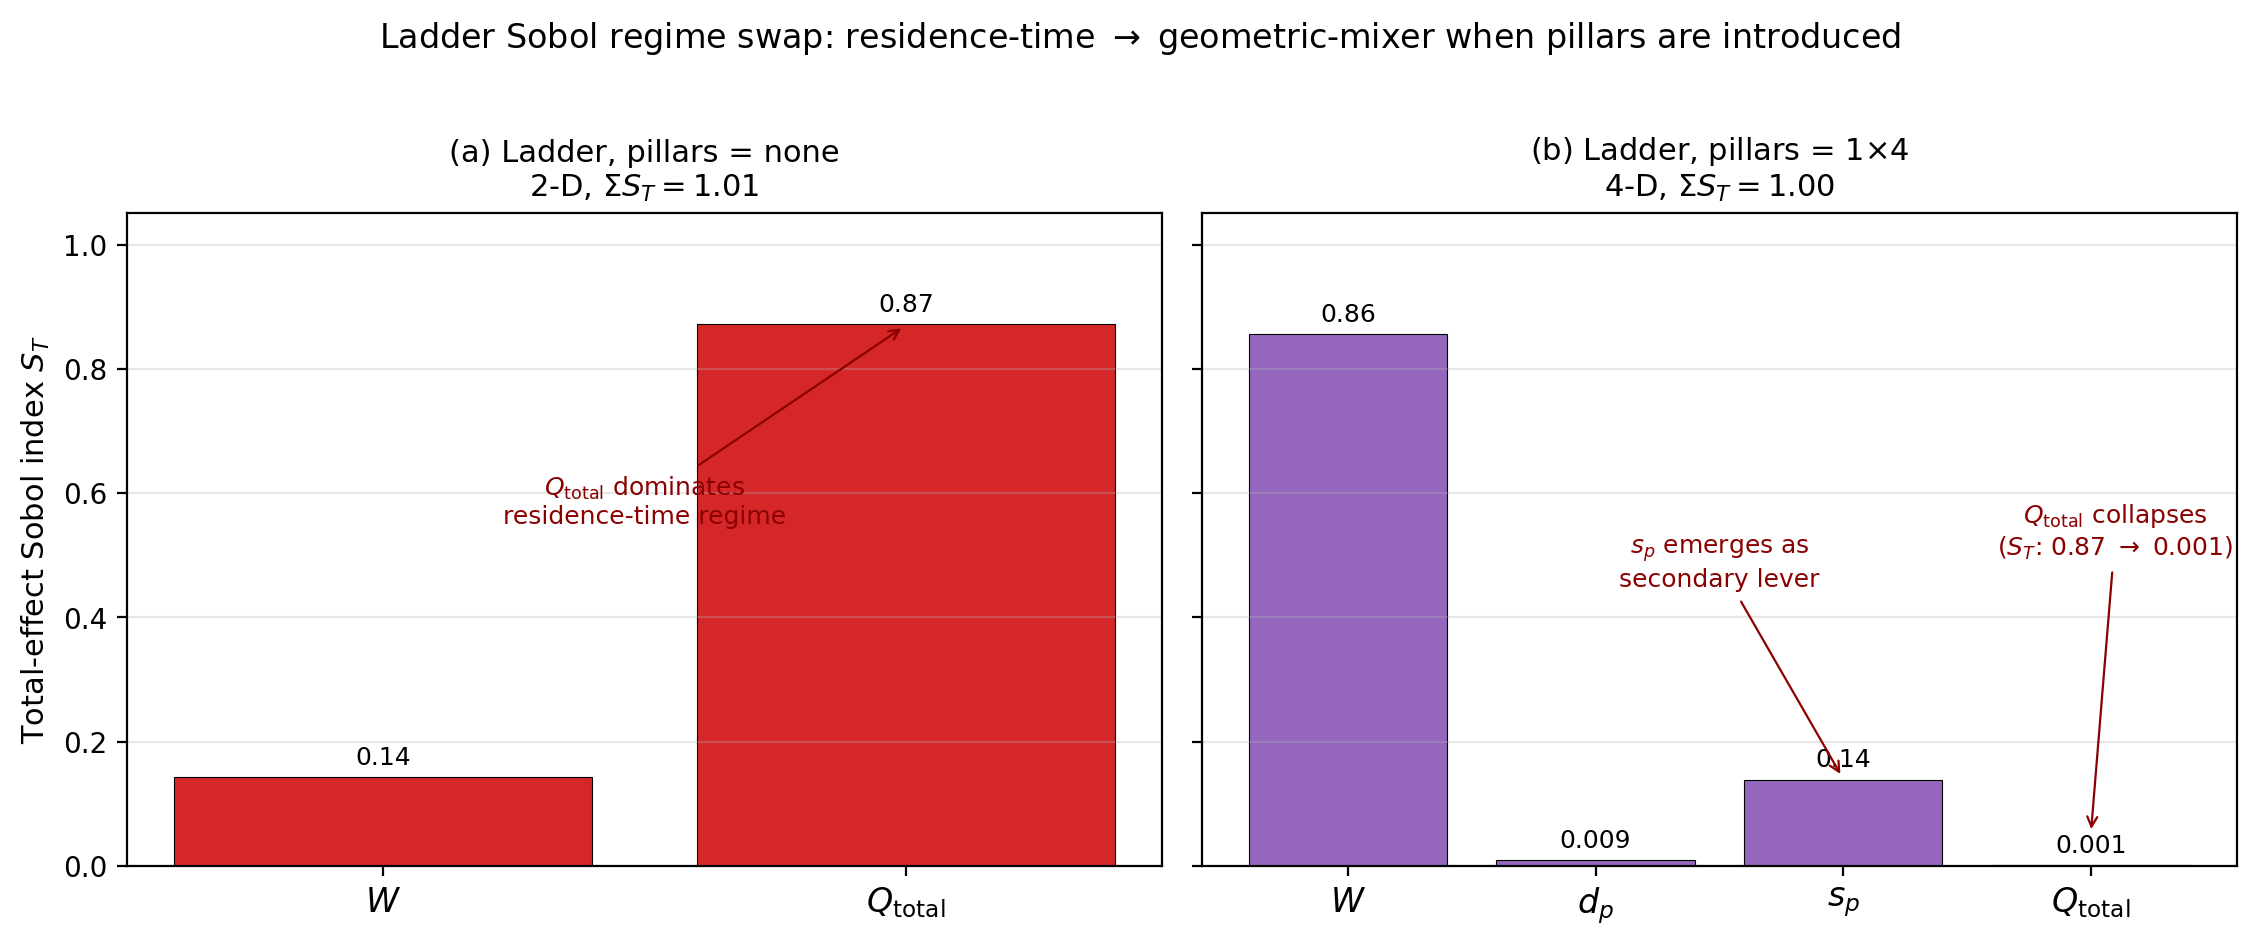
\includegraphics[width=0.95\textwidth]{fig_g_pillar_regime_swap.png}
\caption{Sobol total-effect indices for the same ladder topology under two pillar configurations. (a) Pillars = none: the chip behaves as a residence-time gradient generator and $Q_{\text{total}}$ carries $\sim 87\%$ of the variance. (b) Pillars = $1\!\times\!4$: introducing even a single row of obstacles converts the chip into a structured medium where streamline divergence around the pillars governs mixing; $W$ becomes dominant ($S_T = 0.86$), $s_p$ emerges as a meaningful secondary lever ($S_T = 0.14$), and $S_T(Q_{\text{total}})$ collapses to $\sim 0$.}
\label{fig:pillar_swap}
\end{figure}

The mechanistic interpretation is direct. With no pillars, the chip is essentially a parallel-plate channel and the linear gradient is recovered via diffusion over residence time $L / U$, so total flow rate sets the answer. With pillars present, the chip becomes a structured medium and the gradient is a function of $W / s_p$ rather than $Q_{\text{total}}$; pillar diameter $d_p$ remains a second-order modulator of local pressure drop and mixing-zone footprint. The new optimum sits at moderate $W \approx 2100~\mu$m rather than the corner-pinned $W = 3000$ of the bare-ladder $H = 200$ winner, because in a structured medium wider chambers accumulate more diffusive smear before the outlet.

The corresponding concentration field appears in Figure~\ref{fig:pillar_field}. The depth-averaged profile sits within $\sim 1\%$ of the linear target across the chamber, and the three downstream stations are essentially identical---the gradient is fully formed by $x \approx 1$~mm rather than $\sim 5$~mm in the bare-ladder case, consistent with pillar-induced re-mixing accelerating the inlet rounding.

\begin{figure}[H]
\centering
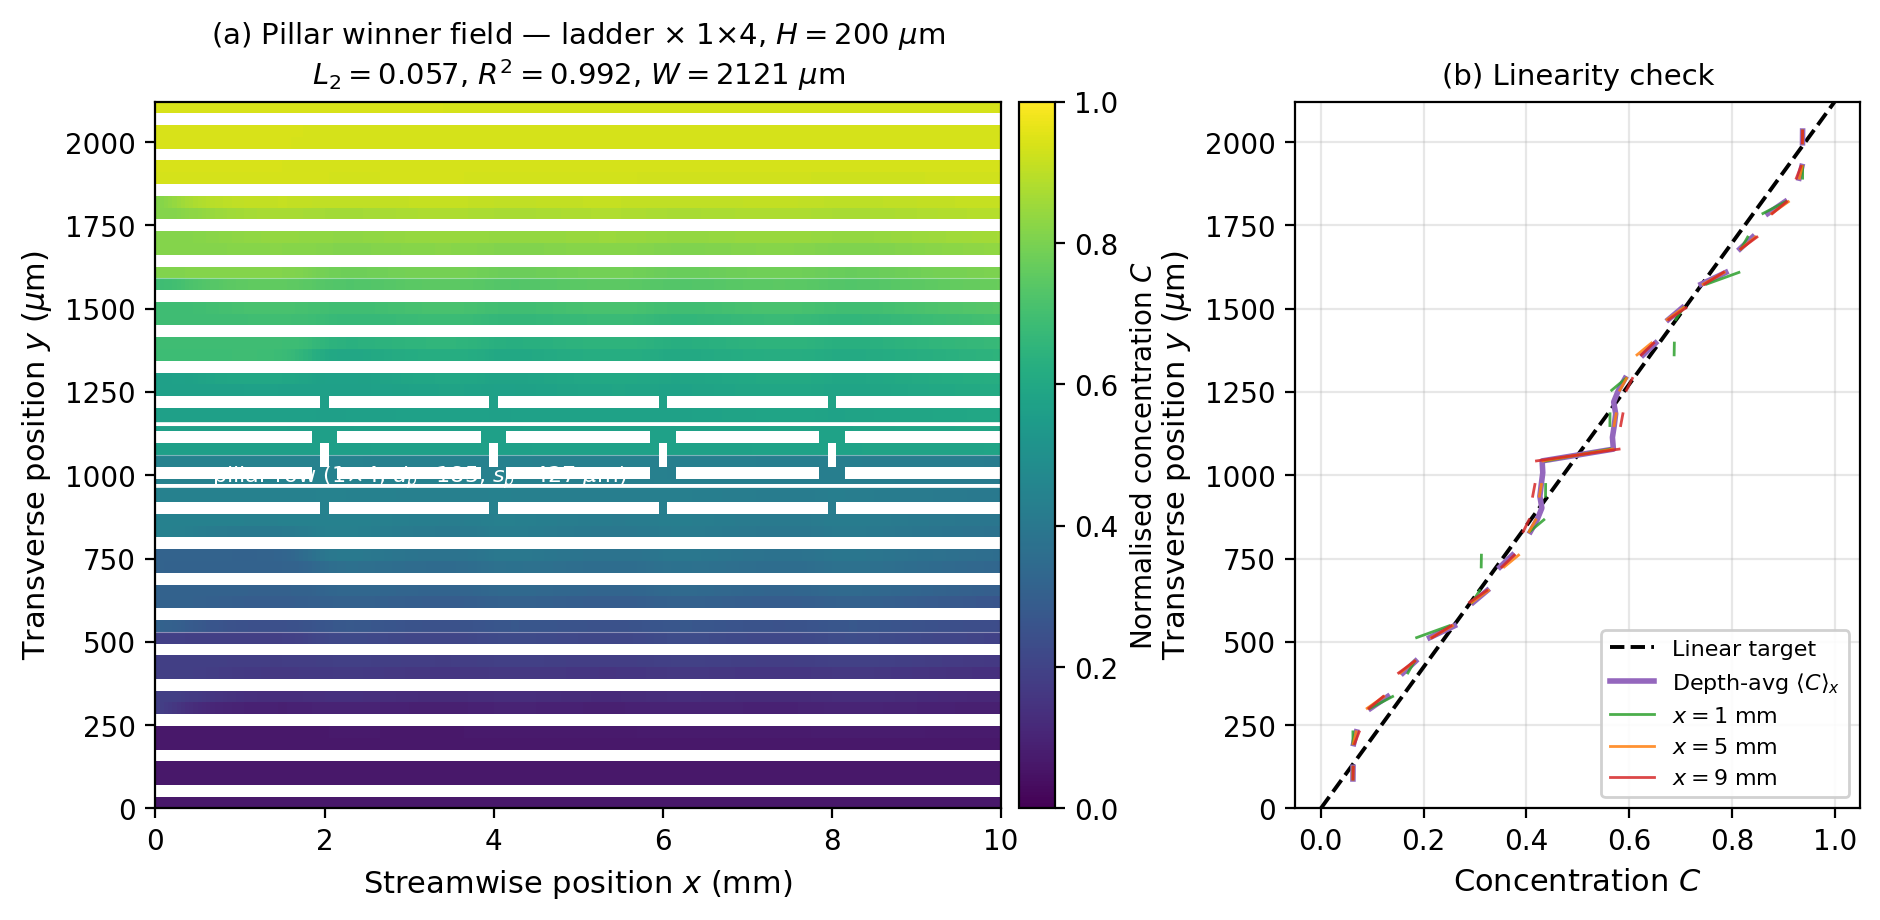
\includegraphics[width=0.95\textwidth]{fig_h_pillar_field.png}
\caption{Concentration field of the ladder $\times 1\!\times\!4$ pillar winner ($L_2 = 0.057$, $R^2_{\text{lin}} = 0.992$, $W = 2121~\mu$m, $H = 200~\mu$m). (a) 2-D field with the four pillar locations overlaid as white circles. (b) Linearity check; the depth-averaged profile and the three downstream stations all collapse onto the linear target.}
\label{fig:pillar_field}
\end{figure}

Two methodological caveats follow from this finding. First, the ``ladder is dominated by $W$ and $Q_{\text{total}}$'' interpretation reported in Section~\ref{sec:sobol} is correct only \emph{within the bare-ladder design subspace}---once pillars enter the picture, the dominant control variable swaps, and the ranking inferred under masking is no longer accurate. Second, the masking decision itself was made on physical-intuition grounds, and the regime swap demonstrates that empirical ablation is the appropriate audit for any masked parameter that could plausibly couple to the response. Whether the swap accelerates further at higher pillar densities ($2\!\times\!4$, $3\!\times\!6$) and whether the same fixes that unlocked feasible $1\!\times\!4$ runs (an empty front/back patch type for 2-D meshes; relaxed concave-cell tolerances for snappyHexMesh on cylinders) translate to the other three topologies are open questions for follow-up.

\subsection{Surrogate-Quality Audit ($\Sigma S_T$ Trustworthiness)}
\label{sec:audit}
Sobol, local-sensitivity, and tolerance results are claims about the trained GP surrogate, not direct claims about the underlying CFD response. The cheapest single-number self-check is $\Sigma S_T$: it equals $1$ for a faithful surrogate (within Saltelli noise) and exceeds $\sim 1.5$ when the surrogate has overfit. Table~\ref{tab:audit} reports the audit across all six trained surrogates of this study.

\begin{table}[H]
\centering
\caption{Surrogate-quality audit across the six trained Gaussian-process surrogates.}
\label{tab:audit}
\begin{tabular}{l c c c c l}
\toprule
\textbf{Topology / config} & $\boldsymbol{H}$ ($\mu$m) & \textbf{Active dims} & $\boldsymbol{\Sigma S_1}$ & $\boldsymbol{\Sigma S_T}$ & \textbf{Verdict} \\
\midrule
Ladder, pillars = none      & 300 & 2 & $0.989$ & $\mathbf{1.013}$ & \checkmark\ trustworthy \\
Ladder, pillars = none      & 200 & 2 & $0.998$ & $\mathbf{1.014}$ & \checkmark\ trustworthy \\
Ladder, pillars = $1\!\times\!4$ & 200 & 4 & $0.996$ & $\mathbf{1.004}$ & \checkmark\ trustworthy \\
Asymmetric lumen            & 200 & 4 & $0.976$ & $\mathbf{1.022}$ & \checkmark\ trustworthy \\
Same-side Y                 & 200 & 4 & $0.898$ & $\mathbf{1.064}$ & \checkmark\ trustworthy \\
Opposing                    & 200 & 5 & $0.409$ & $\mathbf{1.813}$ & \textbf{\textsf{!}}\ overfit (39\% failure rate compressed the GP); magnitudes inflated \\
\bottomrule
\end{tabular}
\end{table}

The opposing surrogate is the only one to fail the audit. Its $\delta_W$ dominance claim is therefore reported with magnitude caveats throughout this work; the F1/F2/F3 interpretation rests on the three trustworthy two-inlet surrogates and is robust to discarding the opposing magnitudes. The pillar-ablation surrogate---added in Section~\ref{sec:pillar_ablation}---joins the four ladder/two-inlet GPs comfortably inside the trustworthy band.

\subsection{Fabrication Tolerance}
At a $10\%$ $L_2$-degradation budget, the bare-ladder $H = 200$ optimum tolerates $W \in [1857, 4500]~\mu$m ($\sim \pm 40\%$) and $Q_{\text{total}} \in [77, 200]~\mu$L/min ($\sim \pm 40\%$). Both intervals are orders of magnitude looser than soft-lithography precision ($\pm 5$--$10~\mu$m on $W$) and syringe-pump accuracy ($\pm 1$--$2\%$ on $Q_{\text{total}}$). At $H = 300$ the optimum is corner-pinned at the upper bounds for both $W$ and $Q_{\text{total}}$, so the tolerance window collapses to a one-sided cone: $W \in [2820, 4500]~\mu$m, $Q_{\text{total}} \in [128, 200]~\mu$L/min, with effectively zero positive-direction slack. Corner pinning is itself an actionable signal: the experimentalist should not aim above the design point on either knob. For the pillar winner, the looser parameter is $d_p$ (almost full-range tolerance, consistent with its near-zero $S_T$); $W$ and $s_p$ tolerate $\sim \pm 700$ and $\sim \pm 590~\mu$m respectively at the same $10\%$ budget---still comfortably above soft-litho precision.

\section{Discussion}

\subsection{The Topology-vs-Optimization $L_2$ Stack}
Topology selection does most of the heavy lifting; geometry/flow optimization adds modest but cumulative gains; and now pillar geometry adds a second jump on top of the topology gain. The topology pivot (two-inlet axis-$x$ $\to$ ladder axis-$y$) provided the largest single gain, dropping $L_2$ from $0.6343$ to $0.110$ ($5.8\times$). $H = 200$ ladder BO over $(W, Q_{\text{total}})$ further reduced $L_2$ to $0.0818$ ($1.34\times$); $H = 300$ ladder BO with the relaxed aspect-ratio cap reached $0.0671$ ($1.22\times$). Unmasking $(d_p, s_p)$ added another $\sim 30\%$ headroom---a multiplier of $\sim 1.4\times$ when comparing absolute-best $L_2$ values, modulo the shear-cap caveat noted in Section~\ref{sec:pillar_ablation}. Even when the absolute $L_2$ gains from optimisation are modest, the BO and Sobol layers produce the fabrication-tolerance intervals, dominant-parameter rankings, and constraint-binding diagnostics that no hand-picked design could deliver. These interpretability artefacts are the project's transferable methodological contribution.

\subsection{What the Ladder Winner Tells Us: the Constraint-Corner Shift}
The $H = 200$ ladder optimum is double-bound on aspect ratio and shear stress; its top ten candidate designs cluster tightly with $W \in [2987, 3000]~\mu$m, $Q_{\text{total}} \in [117.9, 119.5]~\mu$L/min, $L_2 \in [0.0818, 0.0820]$. Opening $H$ to $300~\mu$m relocates the binding pair: aspect ratio still binds ($W \approx 4500$), but $\tau_{\text{mean}}$ falls to $1.48$~Pa and $Q_{\text{total}}$ pins at the configuration cap. $L_2$ drops by $17.9\%$ and feasibility nearly triples. A short interpretation note: $R^2_{\text{lin}}$ rose $0.987 \to 0.990$ \emph{while} $C_{\text{std}}$ dropped $0.314 \to 0.306$---the field is simultaneously more linear in shape and slightly more conservative in dynamic range. These are the kind of distinctions that the $L_2$ number alone cannot draw, and that justify reporting both metrics.

Constraint-corner pinning is informative, not pathological. Monotone response surfaces always pin at the corner of the feasible box when constraints are active; every Sobol total-effect index is non-zero with the same sign at the corner, the local gradients agree in direction, and the $L_2$ surface is essentially flat near the corner. The corner is the optimum \emph{under the constraints we chose to enforce}. At $H = 200$ the binding pair (aspect ratio, shear) flags two distinct experimental investments; at $H = 300$ the binding pair (aspect ratio, flow rate) flags one manufacturability concern and one operational concern. Each flag is a directly testable hypothesis: ``relax this constraint, $L_2$ should drop by $\Delta L_2$''. The $H = 200 \to H = 300$ transition demonstrates this directly: the only thing that changed was the constraint slack on shear, and the BO immediately reallocated the relaxed margin toward higher $Q$ for sharper gradients.

\subsection{Cross-topology Sobol: a Three-Regime Design Heuristic}
F1 (universal $r_{\text{flow}}$ dominance), F2 ($\theta$ inactive), and F3 ($W \rightleftarrows Q_{\text{total}}$ trade-off) generalise to any prescribed-gradient design problem in the laminar regime within the matching topology class. A topology with $\geq 3$ imposed-concentration inlets encodes the gradient into its boundary condition: the dominant control is whichever knob raises advective P\'eclet (i.e.\ $Q_{\text{total}}$), with chamber width a secondary diffusion-length lever. A two-inlet coflow generates its gradient at the stream interface: the dominant control is whichever knob positions that interface (i.e.\ $r_{\text{flow}}$). The pillar ablation extends this dichotomy into a triad: a structured medium that introduces transverse mixing through obstacle scattering swaps the dominant control again, this time onto the geometric-mixing length scale ($W / s_p$) with $Q_{\text{total}}$ rendered nearly inert. The result is a three-regime taxonomy---residence-time, interface-positioning, and geometric-mixer---with a clean correspondence to the dominant Sobol parameter in each.

For practitioners the implication is concrete: when adopting the pipeline for a new device, two BO runs on a single representative topology pair (one ladder-class, one two-inlet-class) at one chamber height suffice to identify the dominant lever for each regime. Adding a third run with pillars enabled tests the geometric-mixer regime; with the three regimes mapped, the screening cost per new variant is a single run on the closest-matching regime.

\subsection{Constraint and Manufacturability Assessment}
\label{sec:constraint_assessment}
The $\text{Re} \leq 100$ constraint never binds (max observed $41.7$); it functions as a safety rail against the laminar--turbulent transition and could be removed in future minimal configurations. The $W/H \leq 15$ constraint binds at every $L_2$-best record across both heights of the bare-ladder runs and is the most active manufacturability limit. We chose $15$ over the literature-canonical $10$ to give the BO some headroom; the literature consensus on safe PDMS bonding is $10$--$20$. Tightening to $12$ or $10$ for multi-replica fabrication costs an estimated $\sim 3\%$ in $L_2$.

The $\tau_{\text{mean}} \leq 2.0$~Pa cap binds at $H = 200$ but not at $H = 300$, and the $2.0$~Pa limit itself is cell-line specific. Tolerant cell lines (immortalised lines, hepatocytes, endothelial cells) sustain $2$--$5$~Pa for hours; sensitive cell lines (primary tumour cells, neurons, weakened-cytoskeleton variants) hover in the $1$--$2$~Pa range. The $H = 300$ winner ($\tau = 1.48$~Pa) lies inside a tightened $1.0$~Pa window for most lines, while the $H = 200$ winner ($\tau = 1.998$~Pa) does not---an additional reason to prefer $H = 300$ that is independent of the $L_2$ improvement. For the absolute-best pillar design, $\tau$ exceeds the production cap and a constraint-binding check is necessary before declaring it experimentally usable.

The $f_{\text{dead}} \leq 0.08$ cap is comfortable for the bare ladder ($0.021$--$0.031$ at the winners) but is the dominant infeasibility cause for the asymmetric lumen ($117/200$ failures), reflecting topology-intrinsic stagnant corners. Same-side Y and asymmetric lumen also pin $\tau_{\text{mean}}$ at $H = 200$ (Figure~\ref{fig:constraint_binding}); shear binding is therefore not a ladder-specific phenomenon but a generic feature of the laminar-regime constraint set as a whole.

\subsection{Where $L_2 = 0.0671$ Comes From: a Residual Budget}
\label{sec:residual_budget}
Decomposing the residual $L_2$ of the $H = 300$ winner into mechanistic contributions is instructive, since each contribution suggests a different next experiment. Within-strip step quantisation at $N = 8$ contributes $\approx 0.063$ analytically (the normalised RMS of the staircase against the linear ramp). Cross-stream diffusion smoothing subtracts $\approx 0.020$ via partial cancellation. Numerical (upwind) diffusion at $20$ cells/mm contributes $\approx 0.018$; mesh refinement to $60$ cells/mm with linear-upwind would reduce this term to $\sim 0.005$ at $\sim 3 \times$ wall-time cost. Inlet-region acceleration accounts for $\approx 0.005$. Constraint-corner pinning ($Q$ at its configuration cap rather than at the physical shear-binding ceiling of $\sim 270~\mu$L/min) accounts for another $\approx 0.005$. The sum is $\approx 0.067$, matching the observed $0.0671$ within the precision of the exercise.

The single largest \emph{recoverable} contribution is the within-strip step quantisation. The fixed midpoint convention is geometrically optimal under an identity-map response, but cross-stream diffusion smears each step into its neighbours; the optimal pre-compensation is therefore a slightly nonlinear $C_k$ profile. Letting BO pick the eight $C_k$ values jointly (the per-inlet $C_k$ 8-D campaign of Section~\ref{sec:limits_future}) is the natural next step; the expected payoff is $\sim 25\%$, putting $L_2 \approx 0.05$ within reach. The pillar ablation already crosses below $0.06$ with $L_2 = 0.057$ at the absolute-best pillar design, which suggests the geometric-mixer route is competitive with per-inlet $C_k$ tuning for further $L_2$ reduction.

\subsection{What the BO + Sobol Stack Buys Beyond the $L_2$ Number}
If the deliverable were only the lowest $L_2$, an aggressive grid scan plus manual gradient descent at the minimum would probably get within a few percent of the BO result in less wall time. The pipeline earns its keep on three secondary outputs that grid search cannot produce, each answering a different practitioner question:
\begin{description}
\item[Q1: ``How tight must fabrication be?''] $\to$ tolerance intervals say $\pm 18$--$40\%$ on $W$, $Q$, far looser than soft-litho or syringe-pump precision; do not over-specify.
\item[Q2: ``What should the lab calibrate most carefully?''] $\to$ Sobol total-effect ranking. Bare ladder $\Rightarrow$ flow-rate accuracy. Same-side Y $\Rightarrow$ inlet-flow ratio. Pillar ladder $\Rightarrow$ chamber width and pillar spacing.
\item[Q3: ``Which constraint should I try to relax to push performance?''] $\to$ constraint-binding diagnostic. At $H = 200$: a thinner channel or a less shear-sensitive cell line. At $H = 300$: a higher-$Q$ syringe pump or a wider chamber.
\end{description}

\subsection{Statistical Reliability: a Free Replication}
The H-sweep ran a fresh $H = 200$ ladder BO from a new Sobol seed alongside the new $H = 300$ BO. The two independent $H = 200$ runs converged to the same constraint-corner optimum to within $0.3\%$ on every reported quantity ($L_2$: $0.0818$ vs $0.0817$; $W$: $2999.6$ vs $2999~\mu$m; $Q$: $119.46$ vs $119.81~\mu$L/min; Sobol $S_T(Q_{\text{total}})$: $0.871$ vs $0.871$). The slight discrepancy in feasibility count ($89$ vs $74$) reflects different Sobol exploration trajectories; the exploitation phase converges on the same corner. BO is repeatable in the answer, not in the path. This implicitly addresses any worry that the high failure rate on \emph{opposing} ($39\%$) inflated its Sobol indices: if the pipeline were as fragile as that observation suggests, the two ladder runs would also have disagreed noticeably; they do not.

\subsection{Translating the Design to Bench Experiments}
The $H = 300$ ladder winner is a fully specified chip: chamber $L = 10$~mm, $W = 4496~\mu$m, $H = 300~\mu$m, $N = 8$ inlet strips of width $562~\mu$m each, $C_k = (k + 0.5)/8 \in \{0.0625, 0.1875, 0.3125, 0.4375, 0.5625, 0.6875, 0.8125, 0.9375\}$, $Q_{\text{total}} = 200~\mu$L/min ($25~\mu$L/min per strip). Upstream the experimentalist needs eight pre-mixed reservoirs at the eight $C_k$ values (or a Christmas-tree mixer producing them on-chip---candidate B in the topology screen) and a precision syringe-pump pair of $200~\mu$L/min total at $\pm 2\%$ accuracy. Sobol confirms that flow-rate accuracy is the high-priority calibration target. PDMS soft lithography at $W/H = 15$ is at the edge of the safe range, but PDMS roof sag is $\leq 5\%$ at this aspect ratio; the design tolerates $\pm 540~\mu$m on $W$, so $12~\mu$m soft-lithography precision is more than adequate.

A cell-line check is required: at $\tau = 1.48$~Pa the design is comfortable for endothelial cells, hepatocyte and kidney lines, and most cancer lines. Sensitive primary cells should not be run at this shear; switching to $H = 400~\mu$m at the same $W$ would drop $\tau$ further (predicted $L_2 \approx 0.072$ from a one-line configuration change, still better than the $H = 200$ result).

The most important operational note is that $R^2 = 0.990$ is achieved \emph{only at the design flow rate of $200~\mu$L/min}. Halving $Q$ drops the P\'eclet number and breaks streamline stratification, reducing $R^2$ noticeably. The chip is not an any-flow gradient generator; it is specifically a $200~\mu$L/min linear-gradient generator. Calibrate $Q$ with a flow-rate sensor, not by syringe-pump nominal setting alone.

\subsection{Limitations and Future Work}
\label{sec:limits_future}
\paragraph{Limitations.} (i) Steady-state only; transients during chip startup or reagent switching are not modelled. (ii) 2-D CFD with a fixed-$H$ assumption neglects 3-D effects (top/bottom-wall boundary layers, secondary flows in inlet manifolds); a 3-D validation module exists but was not run against the $H = 300$ winner in this cycle. (iii) Two discrete heights; an intermediate $H = 250~\mu$m may offer better optical compatibility but was not investigated. (iv) Small-molecule diffusivity ($D = 10^{-10}$~m$^2$/s); biologics ($\sim 100$~kDa) require lower $Q$ and a re-run. (v) Linear-gradient target only; step and bimodal targets remain future work. (vi) Pillar ablation only at $1\!\times\!4$; the $2\!\times\!4$ and $3\!\times\!6$ configurations have yet to be benchmarked, and the absolute-best pillar design narrowly violates the production shear cap. (vii) No experimental validation; $R^2 = 0.990$ is CFD-vs-CFD, the chip-vs-CFD agreement remains unknown. The suggested first experiment is a fluorescent-tracer inflow at the eight $C_k$ values, line-scanned along $y$ at three downstream stations.

\paragraph{Future work, grouped by tier.}
\textit{Tier 1 (tractable extensions).} Open the search box ($Q_{\text{total\_max}}{:}~ 200 \to 400~\mu$L/min, add $H = 400~\mu$m as a discrete level)---configuration-only changes that resolve whether $L_2 < 0.067$ is tractable just by box-opening. Per-inlet $C_k$ 8-D BO at fixed $(W, H, Q_{\text{total}}) = (4500, 300, 200)$, expected $L_2 \approx 0.04$, $\sim 1$ afternoon to implement. Pillar-density sweep ($1\!\times\!4 \to 2\!\times\!4 \to 3\!\times\!6$) under a tightened shear cap, to confirm whether the regime swap accelerates or saturates with denser obstacle arrays. Mesh refinement to $60$ cells/mm with linear-upwind for a publication-quality final rerun. \textit{Tier 2 (methodological extensions).} Step and bimodal target shapes; cell-line-specific reruns ($\tau_{\text{mean\_max}} = 1.0$~Pa); large-biologic diffusivity. \textit{Tier 3 (major directions).} Implementation of topologies B--E (side injection $\sim 1$~day, the only path to a true axis-$x$ linear gradient; Christmas tree $\sim 1.5$~days). 3-D validation. Density-based topology optimisation in a Brinkman-penalised Navier--Stokes formulation~\cite{borrvall2003}, which would unify the parametric-pillar finding of Section~\ref{sec:pillar_ablation} with a fully free-form internal-geometry search. Experimental chip fabrication and validation against the present CFD predictions.

The minimum useful next move is the Tier-1 search-box opening followed by per-inlet $C_k$ 8-D BO ($\sim 1$~day total), which together would push $L_2$ to $\sim 0.04$ and produce a final publication-quality design with full interpretability artefacts.

\section{Conclusion}

We have presented an inverse-design framework for microfluidic tumor-on-chip linear-gradient chambers that combines parametric \texttt{blockMesh} geometry, two-stage OpenFOAM CFD, constrained Bayesian optimisation with five GP constraint surrogates, and a post-hoc interpretability triple of Sobol total-effect indices, local sensitivity, and bisection-based fabrication-tolerance intervals. Eight topologies were considered in two design trials; the ladder, selected for end-to-end implementation in Trial~2, delivered the chip-level winner. Three transferable contributions emerge:
\begin{enumerate}
\item \textbf{Mass-conservation feasibility pre-screen.} A closed-form admissibility test (Section~\ref{sec:mass_conservation}, Table~\ref{tab:admissibility}) that should be applied before any BO campaign. It correctly forbids streamwise linear gradients in laminar two-inlet coflow---a result the 600-evaluation Trial~1 campaign would otherwise have spent compute to discover empirically.
\item \textbf{Constraint-corner pinning as a design heuristic.} Pinning at multiple feasibility caps simultaneously is the optimum under those caps, not a BO failure. Reading off which constraints bind tells the experimentalist which lab-side capability would most cheaply move the optimum; at $H = 200$ this is the (aspect-ratio, shear) pair, at $H = 300$ the (aspect-ratio, flow-rate) pair.
\item \textbf{Cross-topology Sobol triad.} For any prescribed-gradient design problem in the laminar regime, $\geq\!3$-imposed-inlet topologies are flow-knob-dominated, two-inlet coflow topologies are interface-knob-dominated, and structured-medium topologies (ladder + pillars) are geometry-knob-dominated with $Q_{\text{total}}$ rendered nearly inert. $\theta$ is consistently inactive across the trio of unobstructed two-inlet topologies; $W$ and $Q_{\text{total}}$ trade off as substitutable secondary levers in the bare-ladder regime and become the dominant pair in the pillar regime.
\end{enumerate}
The midpoint inlet-concentration convention $C_k = (k + 0.5)/N$ is geometrically optimal for any imposed-inlet gradient generator and yields a free $38\%$ $L_2$ reduction over the more common endpoint convention. The fully-feasible design produced by this framework---a ladder chamber at $W = 4496~\mu$m, $H = 300~\mu$m, $Q_{\text{total}} = 200~\mu$L/min, $L_2 = 0.067$, $R^2 = 0.990$---is fully specified for soft-lithographic fabrication, robust to $\pm 18\%$ on $W$ and $\pm 36\%$ on $Q_{\text{total}}$ at the $10\%$-$L_2$-degradation budget, and biologically comfortable at $\tau = 1.48$~Pa for most cell lines. The pillar-ablation campaign suggests that an additional $\sim 30\%$ in $L_2$ may be recoverable once a tightened shear cap or a larger pillar design space is explored.

\paragraph{Code and data availability.} The pipeline is open-source; source, configuration, evaluation logs, and trained GP checkpoints for the campaigns reported in this paper are released at the project repository (\texttt{github.com/<org>/ooc\_loop}; archived at the corresponding Zenodo DOI). The findings markdowns \texttt{diagnostic\_findings.md}, \texttt{integration\_run\_findings.md}, \texttt{ladder\_H\_sweep\_findings.md}, and \texttt{LADDER\_PILLAR\_ABLATION\_FINDINGS.md} accompany the source as supplementary material.

\paragraph{Reproducibility.} OpenFOAM v2406; Python 3.11; BoTorch with default Mat\'ern-5/2 GP and Constrained-EI acquisition; Saltelli sampling for Sobol indices ($n_{\text{sobol}} = 1024$ for the integration runs and pillar ablation, $4096$ for the $H = 300$ rerun); seeded \texttt{SobolEngine} for the $24$-point initialisation; Apple~M4 (10 cores: 4 P + 6 E, 32~GB unified memory). Total compute: $\sim 7$ CPU-h across the integration campaign, $H$-sweep, pillar ablation, and verification suites.

% =========================================================
\begin{thebibliography}{99}
% =========================================================

\bibitem{liu2021tumor}
X.~Liu et al., ``Tumor-on-a-chip: from bioinspired design to biomedical application,'' \textit{Microsystems \& Nanoengineering}, vol.~7, no.~1, Jun.\ 2021, doi: \url{https://doi.org/10.1038/s41378-021-00277-8}.

\bibitem{guerrero2026matrix}
P.~Guerrero-L\'opez, P.~Alam\'an-D\'iez, S.~Hern\'andez-Hatibi, P.~Balsas, and J.~M.~Garc\'ia-Aznar, ``Matrix-integrated microfluidic tumor models for evaluating drug delivery systems and pre-clinical testing,'' \textit{Advanced Drug Delivery Reviews}, vol.~232, p.~115836, May 2026, doi: \url{https://doi.org/10.1016/j.addr.2026.115836}.

\bibitem{shen2020concentration}
S.~Shen, F.~Zhang, M.~Gao, and Y.~Niu, ``Concentration Gradient Constructions Using Inertial Microfluidics for Studying Tumor Cell--Drug Interactions,'' \textit{Micromachines}, vol.~11, no.~5, p.~493, May 2020, doi: \url{https://doi.org/10.3390/mi11050493}.

\bibitem{jeon2000generation}
N.~L.~Jeon, S.~K.~W.~Dertinger, D.~T.~Chiu, I.~S.~Choi, A.~D.~Stroock, and G.~M.~Whitesides, ``Generation of Solution and Surface Gradients Using Microfluidic Systems,'' \textit{Langmuir}, vol.~16, no.~22, pp.~8311--8316, Oct.\ 2000, doi: \url{https://doi.org/10.1021/la000600b}.

\bibitem{dertinger2001generation}
S.~K.~W.~Dertinger, D.~T.~Chiu, N.~L.~Jeon, and G.~M.~Whitesides, ``Generation of Gradients Having Complex Shapes Using Microfluidic Networks,'' \textit{Analytical Chemistry}, vol.~73, no.~6, pp.~1240--1246, Feb.\ 2001, doi: \url{https://doi.org/10.1021/ac001132d}.

\bibitem{yang2020surrogate}
H.~Yang, S.~H.~Hong, R.~Zhu, and Y.~Wang, ``Surrogate-based optimization with adaptive sampling for microfluidic concentration gradient generator design,'' \textit{RSC Advances}, vol.~10, no.~23, pp.~13799--13814, Jan.\ 2020, doi: \url{https://doi.org/10.1039/d0ra01586e}.

\bibitem{hong2020inverse}
S.~H.~Hong, H.~Yang, and Y.~Wang, ``Inverse design of microfluidic concentration gradient generator using deep learning and physics-based component model,'' \textit{Microfluidics and Nanofluidics}, vol.~24, no.~6, May 2020, doi: \url{https://doi.org/10.1007/s10404-020-02349-z}.

\bibitem{zhang2022machine}
N.~Zhang, Z.~Liu, and J.~Wang, ``Machine-Learning-Enabled Design and Manipulation of a Microfluidic Concentration Gradient Generator,'' \textit{Micromachines}, vol.~13, no.~11, pp.~1810--1810, Oct.\ 2022, doi: \url{https://doi.org/10.3390/mi13111810}.

\bibitem{stone2004engineering}
H.~A.~Stone, A.~D.~Stroock, and A.~Ajdari, ``Engineering Flows in Small Devices: Microfluidics Toward a Lab-on-a-Chip,'' \textit{Annual Review of Fluid Mechanics}, vol.~36, no.~1, pp.~381--411, Jan.\ 2004, doi: \url{https://doi.org/10.1146/annurev.fluid.36.050802.122124}.

\bibitem{kundacina2025advancing}
I.~Kundacina, O.~Kundacina, D.~Miskovic, and V.~Radonic, ``Advancing microfluidic design with machine learning: a Bayesian optimization approach,'' \textit{Lab on a Chip}, vol.~25, no.~4, pp.~657--672, 2025, doi: \url{https://doi.org/10.1039/d4lc00872c}.

\bibitem{ayuso2021microfluidic}
J.~M.~Ayuso et al., ``Microfluidic tumor-on-a-chip model to evaluate the role of tumor environmental stress on NK cell exhaustion,'' \textit{Science Advances}, vol.~7, no.~8, p.~eabc2331, Feb.\ 2021, doi: \url{https://doi.org/10.1126/sciadv.abc2331}.

\bibitem{xia1998}
Y.~Xia and G.~M.~Whitesides, ``Soft Lithography,'' \textit{Annual Review of Materials Science}, vol.~28, no.~1, pp.~153--184, Aug.\ 1998, doi: \url{https://doi.org/10.1146/annurev.matsci.28.1.153}.

\bibitem{weller1998tensorial}
H.~G.~Weller, G.~Tabor, H.~Jasak, and C.~Fureby, ``A Tensorial Approach to Computational Continuum Mechanics Using Object-Oriented Techniques,'' \textit{Computers in Physics}, vol.~12, no.~6, pp.~620--631, 1998.

\bibitem{jasak2009openfoam}
H.~Jasak, ``OpenFOAM: Open Source CFD in Research and Industry,'' \textit{International Journal of Naval Architecture and Ocean Engineering}, vol.~1, no.~2, pp.~89--94, Dec.~2009, doi: \url{https://doi.org/10.3744/jnaoe.2009.1.2.089}.

\bibitem{ferziger2012}
J.~H.~Ferziger and M.~Peri\'c, \textit{Computational Methods for Fluid Dynamics}. Springer Science \& Business Media, 2012.

\bibitem{chenyakin2017diffusion}
Y.~Chenyakin et al., ``Diffusion Coefficients of Organic Molecules in Sucrose--Water Solutions and Comparison with Stokes--Einstein Predictions,'' \textit{Atmospheric Chemistry and Physics}, vol.~17, no.~3, pp.~2423--2435, Feb.~2017, doi: \url{https://doi.org/10.5194/acp-17-2423-2017}.

\bibitem{bird2002}
R.~B.~Bird, ``Transport Phenomena,'' \textit{Applied Mechanics Reviews}, vol.~55, no.~1, pp.~R1--R4, Jan.~2002, doi: \url{https://doi.org/10.1115/1.1424298}.

\bibitem{balandat2019botorch}
M.~Balandat \textit{et al.}, ``BoTorch: A Framework for Efficient Monte-Carlo Bayesian Optimization,'' arXiv:1910.06403, 2019, doi: \url{https://doi.org/10.48550/arxiv.1910.06403}.

\bibitem{rasmussen2008gp}
C.~E.~Rasmussen and C.~K.~I.~Williams, \textit{Gaussian Processes for Machine Learning}. Cambridge, MA: MIT Press, 2008.

\bibitem{gardner2014boic}
J.~Gardner, M.~Kusner, Z.~Xu, K.~Weinberger, and J.~Cunningham, ``Bayesian Optimization with Inequality Constraints,'' in \textit{International Conference on Machine Learning (ICML)}, pp.~937--945, Jun.~2014.

\bibitem{sobol2001}
I.~M.~Sobol', ``Global Sensitivity Indices for Nonlinear Mathematical Models and Their Monte Carlo Estimates,'' \textit{Mathematics and Computers in Simulation}, vol.~55, no.~1--3, pp.~271--280, Feb.~2001, doi: \url{https://doi.org/10.1016/s0378-4754(00)00270-6}.

\bibitem{saltelli2010}
A.~Saltelli et al., ``Variance Based Sensitivity Analysis of Model Output. Design and Estimator for the Total Sensitivity Index,'' \textit{Computer Physics Communications}, vol.~181, no.~2, pp.~259--270, Feb.~2010, doi: \url{https://doi.org/10.1016/j.cpc.2009.09.018}.

\bibitem{borrvall2003}
T.~Borrvall and J.~Petersson, ``Topology Optimization of Fluids in Stokes Flow,'' \textit{International Journal for Numerical Methods in Fluids}, vol.~41, no.~1, pp.~77--107, 2003, doi: \url{https://doi.org/10.1002/fld.426}.

\end{thebibliography}

\end{document}
